\documentclass[a4paper,12pt]{article}

\usepackage{graphicx}
\usepackage{amsfonts}
\usepackage{fancyhdr}
\usepackage{helvet}
\usepackage{courier}
\usepackage{epsfig}
\usepackage{type1cm}
\usepackage{makeidx}        
\usepackage[bottom]{footmisc}
\usepackage[all]{xy}
\usepackage{fancybox}
\usepackage[utf8]{inputenc}    % Acentos en UTF-8
\usepackage[spanish]{babel}    % Órdenes e idioma en español
\usepackage[table]{xcolor}     % Necesario para las filas sombreadas de las tablas
\usepackage{amsmath}
\usepackage{booktabs}
\usepackage{amssymb}
\usepackage{wasysym}
\usepackage{enumerate}
\usepackage{multicol}
\usepackage{enumitem} % Para listas compactas dentro de la tabla
\usepackage{epstopdf}
\usepackage{wrapfig}
\usepackage{pgf,tikz}
\usepackage{subfigure}
\usepackage{bm}
\usepackage{yhmath}
\usepackage{float}
\usepackage[mathscr]{euscript}
\usetikzlibrary{shapes.gates.logic.US,trees,positioning,arrows}

\usepackage{algorithm}
\usepackage{algpseudocode}
\usepackage{amsthm}
\usepackage{tabularx}
\usepackage{mathtools}
\usepackage{multirow}
\usepackage{hyperref}
\usepackage{eso-pic}
\usepackage{colortbl}
\usepackage{hhline}
\usepackage{xltabular}


\hypersetup{colorlinks=true}

\def\proof{\paragraph{}}
\def\endproof{\hfill$\blacksquare$}
\usepackage[table]{xcolor}
\definecolor{verdeApagado}{HTML}{A4BEA7}
\definecolor{azulPastelApagado}{HTML}{ABBBCB}
\definecolor{azulclaro}{HTML}{d1dbe4}
%%%%%%%%%%%%%%%%%%%%%%%%%%%%%%%%%%%%%%%%%%%%%%%%%%%%%%%%%%%%%%%%%%%%%%%%%%%%%%%%%%%%%%%%%%%%%
%% Márgenes
\usepackage{geometry}
\geometry{
top=3cm,
bottom=3cm,
left=3cm,
right=3cm
}

%% Encabezados y pie de página
\pagestyle{fancy}
\fancyhf{}

\lhead{}
\rhead{Metodologías de Desarrollo Ágil}
\renewcommand{\headrulewidth}{0.08pt}

\lfoot{}
\rfoot{DobleM - MDA DGP}
\cfoot{\thepage}
\renewcommand{\footrulewidth}{0.08pt}
%%%%%%%%%%%%%%%%%%%%%%%%%%%%%%%%%%%%%%%%%%%%%%%%%%%%%%%%%%%%%%%%%%%%%%%%%%%%%%%%%%%%%%%%%%%%%%% 
\begin{document}

%%%%%%%%%%%%%%%%%%%%%%%%%%%%%%%%%%%%%%%%%%%%%%%%%%%%%%%%%%%%%%%%%%%%%%%%%%%%%%%%%%%%%%%%%%%%%%%
%%%% Portada:   
% --- IMAGEN DE FONDO DE PORTADA ---
\AddToShipoutPictureBG*{%
  \AtPageLowerLeft{%
    
\includegraphics[width=\paperwidth,height=\paperheight]{img/Fondo_Portada.png}%
  }%
}
\pagestyle{empty}

\begin{center}
    \hspace{-1cm}
    \centering
    
    \vfill
    \begin{figure}[H]
        \centering
        
\includegraphics[width=0.4\textwidth]{img/logo.png}
    \end{figure}
	 \vfill
    {\textsc{\Huge DOBLE-M SOFTWARE}}\\[0.4cm]
	 \vfill
    {\textsc{\large Metodologías de Desarrollo Ágil}} \\[0.2cm]
    {\textsc{\large Dirección y Gestión de Proyectos}}
    
    
    \vfill
	\vfill
	\vfill
    {\Large{Minerva Cebrián Marín}} {(mcm17@correo.ugr.es)} \\
    
    \vfill
    {\Large{Jorge García Gámiz}} {(jorgegarciag@correo.ugr.es)} \\

     \vfill
    {\Large{Cristina García Gázquez}} {(jorgegarciag@correo.ugr.es)} \\

    \vfill
    {\Large{Ángela García Olmos}} {(angelagrc@correo.ugr.es)} \\

    \vfill
    {\Large{Kirsten Gazy Manalo}} {(kirstenmanalo@correo.ugr.es)} \\

    \vfill
    {\Large{Pedro Javier Pérez Jiménez}} {(pjpz@correo.ugr.es)}\\
    
    \vfill
    {\Large{Daniel Vega Jiménez}} {(deltac@correo.ugr.es)} \\
    
    \vfill
	\vfill
    {Curso 2026-2027}
        \vfill
    
    \begin{figure}[H]
        \centering
        
\includegraphics[width=0.2\textwidth]{ugr.png}
    \end{figure}
    \vfill
    {\small }
\end{center} 

%%%%%%%%%%%%%%%%%%%%%%%%%%%%%%%%%%%%%%%%%%%%%%%%%%%%%%%%%%%%%%%%%%%%%%%%%%%%%%%%%%%%%%%%%%%%%%%%%%%

% ---------------- Índice ----------------
\newpage
\pagestyle{fancy}
\setcounter{page}{1}

\makeatletter
\let\ps@plain\ps@fancy
\makeatother

\tableofcontents 
% MDA
 \newpage
\section{Roles del Equipo}

\noindent
\begin{tabularx}{\textwidth}{|>{\columncolor{azulPastelApagado}\bfseries}p{5.5cm}|X|}
\hline
\rowcolor{azulPastelApagado}
\multicolumn{2}{|c|}{\color{white}\textbf{ROLES Y RESPONSABILIDADES}} \\
\hline
Coordinador & DANIEL VEGA JIMÉNEZ\\
\hline
Catalogador & JORGUE GARCÍA GÁMIZ \\
\hline
Moderador & ÁNGELA GARCÍA OLMOS \\
\hline
Presentador & DANIEL VEGA JIMÉNEZ\\
\hline
Gestor de la Calidad & MINERVA CEBRIÁN MARIN\\
\hline
Gestor de usabilidad y \newline accesibilidad & PEDRO JAVIER PÉREZ JIMÉNEZ \\
\hline
\end{tabularx}
\newpage
\newcommand{\colorEncabezado}{azulPastelApagado}
\newcommand{\colorTextoEncabezado}{white}
\newcommand{\colorColumnaIzquierda}{azulclaro}

% Columna especial para multicolumns que abarcan las dos últimas columnas con salto de línea automático
\newcolumntype{Y}{>{\hsize=\dimexpr2\hsize+2\tabcolsep+\arrayrulewidth\relax}X}

\section{Personas y Escenarios}


 %PERSONA 1 TUTOR
\subsection{Persona 1: Tutor}
\noindent
\begin{xltabular}{\textwidth}{|p{3.5cm}|X|p{4cm}|}
\hline
\rowcolor{\colorEncabezado}
\multicolumn{3}{|c|}{%
  \color{\colorTextoEncabezado}\textbf{Tutor}%
} \\
\hline

\cellcolor{\colorColumnaIzquierda}\textbf{Nombre}
& Gema Uceda Cabezali
& \multirow{5}{*}{%
  \parbox{3.8cm}{\centering
    \vspace{0.1cm}
    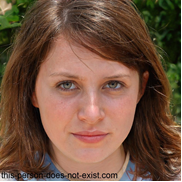
\includegraphics[width=2.6cm, height=2.6cm, keepaspectratio]{img/personas/persona1.png}%
    \vspace{0.1cm}
  }%
} \\
\hhline{|--|~|}

\cellcolor{\colorColumnaIzquierda}\textbf{Edad}
& 37 & \\
\hhline{|--|~|}

\cellcolor{\colorColumnaIzquierda}\textbf{Sexo}
& Mujer & \\
\hhline{|--|~|}

\cellcolor{\colorColumnaIzquierda}\textbf{Discapacidad}
& No tiene & \\
\hhline{|--|~|}

\cellcolor{\colorColumnaIzquierda}\textbf{Educación}
& Estudios universitarios & \\
\hline

\rowcolor{\colorEncabezado}
\multicolumn{3}{|c|}{%
  \color{\colorTextoEncabezado}\textbf{Contexto de uso}%
} \\
\hline

Cuándo
& \multicolumn{2}{Y|}{%
  \small En cualquier momento, utiliza el móvil para tareas cotidianas.%
} \\
\hline

Dónde
& \multicolumn{2}{Y|}{%
  \small En cualquier lugar.%
} \\
\hline

Tipo de ordenador
& \multicolumn{2}{Y|}{%
  \small Principalmente el móvil, aunque también usa el ordenador en el trabajo.%
} \\
\hline

\rowcolor{\colorEncabezado}
\multicolumn{3}{|c|}{%
  \color{\colorTextoEncabezado}\textbf{Misión}%
} \\
\hline

Objetivo
& \multicolumn{2}{Y|}{%
  \small Consultar fácilmente el horario diario de su hijo y ayudarle a organizarlo.%
} \\
\hline

Expectativas
& \multicolumn{2}{Y|}{%
  \small Una interfaz sencilla para programar tareas y consultar sus actividades.%
} \\
\hline

\rowcolor{\colorEncabezado}
\multicolumn{3}{|c|}{%
  \color{\colorTextoEncabezado}\textbf{Motivación}%
} \\
\hline

Urgencia
& \multicolumn{2}{Y|}{%
  \small Cuanto antes.%
} \\
\hline

Deseo
& \multicolumn{2}{Y|}{%
  \small Tranquilidad para ella y para su hijo.%
} \\
\hline

\rowcolor{\colorEncabezado}
\multicolumn{3}{|c|}{%
  \color{\colorTextoEncabezado}\textbf{Actitud hacia la tecnología}%
} \\
\hline

Actitud
& \multicolumn{2}{Y|}{%
  \small Proactiva y capaz de desenvolverse en entornos virtuales nuevos.%
} \\
\hline
\end{xltabular}

\vspace{0.8cm}
%Escenario 1
\noindent
\begin{xltabular}{\textwidth}{|p{3.5cm}|X|p{4cm}|}
\hline
\rowcolor{\colorEncabezado}
\multicolumn{3}{|c|}{%
  \color{\colorTextoEncabezado}\textbf{Escenario 1}%
} \\
\hline

Nombre persona
& Gema Uceda Cabezali
& \multirow{4}{*}{%
  \parbox{3.8cm}{\centering
    \vspace{0.1cm}
    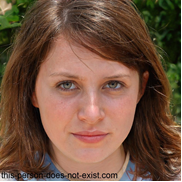
\includegraphics[width=3cm, height=3cm, keepaspectratio]{img/personas/persona1.png}%
    \vspace{0.1cm}
  }%
} \\
\cline{1-2}

Objetivo persona
& \rule{0pt}{2.5cm}Crear una tarea para su hijo & \\
\hline

\rowcolor{\colorEncabezado}
\multicolumn{3}{|c|}{%
  \color{\colorTextoEncabezado}\textbf{Descripción del escenario}%
} \\
\hline

\cellcolor{\colorColumnaIzquierda}\textbf{Descripción}
& \multicolumn{2}{Y|}{%
  \small
  Gema le ha pedido a su hijo que vaya a comprar algo a una
  tienda del vecindario después de salir de clase. Coge el móvil
  y abre la aplicación para añadir la tarea a su agenda.\par\smallskip

  Inicia sesión, accede a la zona de gestión y selecciona el
  perfil de su hijo. Después, elige la opción de añadir una
  tarea, introduce su descripción, la hora de salida del colegio
  y la duración estimada, y confirma la creación.\par\smallskip

  Si no existe ningún conflicto con otras tareas, la aplicación
  incorporará la nueva actividad al calendario. Su hijo podrá
  consultarla al salir de clase.%
} \\
\hline

\end{xltabular}

%Escenario 2
\noindent
\begin{xltabular}{\textwidth}{|p{3.5cm}|X|p{4cm}|}
\hline
\rowcolor{\colorEncabezado}
\multicolumn{3}{|c|}{%
  \color{\colorTextoEncabezado}\textbf{Escenario 2}%
} \\
\hline

Nombre persona
& Gema Uceda Cabezali
& \multirow{4}{*}{%
  \parbox{3.8cm}{\centering
    \vspace{0.1cm}
    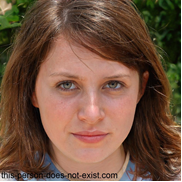
\includegraphics[width=3cm, height=3cm, keepaspectratio]{img/personas/persona1.png}%
    \vspace{0.1cm}
  }%
} \\
\cline{1-2}

Objetivo persona
& \rule{0pt}{2.5cm}Editar una tarea para su hijo & \\
\hline

\rowcolor{\colorEncabezado}
\multicolumn{3}{|c|}{%
  \color{\colorTextoEncabezado}\textbf{Descripción del escenario}%
} \\
\hline

\cellcolor{\colorColumnaIzquierda}\textbf{Descripción}
& \multicolumn{2}{Y|}{%
  \small
  Gema creó una tarea previamente para que su hijo comprara algo en una tienda del vecindario al volver de clases.

En un momento del día, recuerda otra cosa que debe añadir para que su hijo compre, 
se mete en la aplicación logeandose de nuevo y selecciona la tarea previamente añadida. 
Selecciona el botón de edición y modifica la descripción de la tarea. La guarda y ve el cambio reflejado.


} \\
\hline

\end{xltabular}















\newpage

\subsection{Persona 2: Profesor}

 %PERSONA 2 PROFESOR
\noindent
\begin{xltabular}{\textwidth}{|p{3.5cm}|X|p{4cm}|}
\hline
\rowcolor{\colorEncabezado}
\multicolumn{3}{|c|}{%
  \color{\colorTextoEncabezado}\textbf{Profesor}%
} \\
\hline

\cellcolor{\colorColumnaIzquierda}\textbf{Nombre}
& Alejandra Fajardo
& \multirow{5}{*}{%
  \parbox{3.8cm}{\centering
    \vspace{0.1cm}
    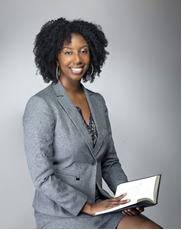
\includegraphics[width=4cm, height=4cm, keepaspectratio]{img/personas/persona2.png}%
    \vspace{0.1cm}
  }%
} \\
\hhline{|--|~|}

\cellcolor{\colorColumnaIzquierda}\textbf{Edad}
& 44 & \\
\hhline{|--|~|}

\cellcolor{\colorColumnaIzquierda}\textbf{Sexo}
& Mujer & \\
\hhline{|--|~|}

\cellcolor{\colorColumnaIzquierda}\textbf{Discapacidad}
& No tiene & \\
\hhline{|--|~|}

\cellcolor{\colorColumnaIzquierda}\textbf{Educación}
& Educación	Universidad – 
Grado en Educación Primaria con mención en Pedagogía Terapéutica (PT)	 & \\
\hline

\rowcolor{\colorEncabezado}
\multicolumn{3}{|c|}{%
  \color{\colorTextoEncabezado}\textbf{Contexto de uso}%
} \\
\hline

Cuándo
& \multicolumn{2}{Y|}{%
  \small Durante la jornada escolar, especialmente al planificar las actividades de la semana, organizar las tareas de los alumnos y consultar qué actividades están previstas para cada día. También puede utilizarlo fuera del horario escolar para preparar y planificar las clases%
} \\
\hline

Dónde
& \multicolumn{2}{Y|}{%
  \small Principalmente en el aula y en la sala de profesores, aunque también puede utilizarlo desde casa para preparar la planificación semanal%
} \\
\hline

Tipo de ordenador
& \multicolumn{2}{Y|}{%
  \small Ordenador portátil o de sobremesa del centro. También podría utilizar ocasionalmente una tableta para consultar rápidamente el calendario durante las clases%
} \\
\hline

\rowcolor{\colorEncabezado}
\multicolumn{3}{|c|}{%
  \color{\colorTextoEncabezado}\textbf{Misión}%
} \\
\hline

Objetivo
& \multicolumn{2}{Y|}{%
  \small Organizar de forma sencilla las actividades, tareas y eventos de sus alumnos mediante un calendario, pudiendo planificar qué debe realizarse cada día y realizar un seguimiento de las actividades pendientes%
} \\
\hline

Expectativas
& \multicolumn{2}{Y|}{%
  \small Espera que la aplicación le permita crear, modificar y consultar tareas fácilmente, organizándolas por alumno y fecha. También espera poder visualizar rápidamente las actividades del día o de la semana y recibir avisos cuando haya tareas o actividades pendientes%
} \\
\hline

\rowcolor{\colorEncabezado}
\multicolumn{3}{|c|}{%
  \color{\colorTextoEncabezado}\textbf{Motivación}%
} \\
\hline

Urgencia
& \multicolumn{2}{Y|}{%
  \small Necesita organizar de forma clara las numerosas actividades y tareas que debe preparar para diferentes alumnos, evitando olvidos y reduciendo el tiempo dedicado a la planificación%
} \\
\hline

Deseo
& \multicolumn{2}{Y|}{%
  \small Quiere tener toda la planificación de sus alumnos organizada en un único lugar, pudiendo saber rápidamente qué tiene que hacer cada día y qué tareas están pendientes para cada alumno%
} \\
\hline

\rowcolor{\colorEncabezado}
\multicolumn{3}{|c|}{%
  \color{\colorTextoEncabezado}\textbf{Actitud hacia la tecnología}%
} \\
\hline

Actitud
& \multicolumn{2}{Y|}{%
  \small Tiene una actitud positiva pero práctica hacia la tecnología. Está dispuesta a utilizar herramientas digitales si le ayudan a organizar mejor su trabajo y ahorrar tiempo. Prefiere aplicaciones sencillas, intuitivas y rápidas, especialmente porque durante la jornada escolar necesita consultar o introducir información sin que esto interfiera demasiado con la atención a los alumnos. Puede sentirse frustrada ante calendarios demasiado complejos o que requieran introducir demasiada información para crear una tarea%
} \\
\hline
\end{xltabular}

\vspace{0.8cm}
%Escenario 1
\noindent
\begin{xltabular}{\textwidth}{|p{3.5cm}|X|p{4cm}|}
\hline
\rowcolor{\colorEncabezado}
\multicolumn{3}{|c|}{%
  \color{\colorTextoEncabezado}\textbf{Escenario 1}%
} \\
\hline

Nombre persona
& Alejandra Fajardo
& \multirow{4}{*}{%
  \parbox{3.8cm}{\centering
    \vspace{0.1cm}
    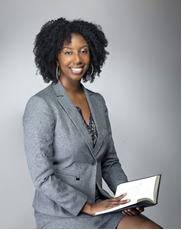
\includegraphics[width=6cm, height=6cm, keepaspectratio]{img/personas/persona2.png}%
    \vspace{0.1cm}
  }%
} \\
\cline{1-2}

Objetivo persona
& \rule{0pt}{2.5cm}Organizar de forma sencilla las actividades, tareas y eventos de sus alumnos mediante un calendario, pudiendo planificar qué debe realizarse cada día y realizar un seguimiento de las actividades pendientes & \\
\hline

\rowcolor{\colorEncabezado}
\multicolumn{3}{|c|}{%
  \color{\colorTextoEncabezado}\textbf{Descripción del escenario}%
} \\
\hline

\cellcolor{\colorColumnaIzquierda}\textbf{Descripción}
& \multicolumn{2}{Y|}{%
  \small
  Alejandra es profesora en un colegio para niños y niñas con discapacidades funcionales. A primera hora de la mañana recibe el aviso de que la excursión prevista para ese día no podrá realizarse debido a la lluvia. La actividad estaba programada en el calendario del colegio y varios alumnos ya estaban preparados para salir.
Alejandra accede a la aplicación para consultar las actividades previstas para ese día y comprueba qué otras actividades estaban programadas para su grupo. Decide reorganizar la jornada y sustituir la excursión por un taller de música que estaba previsto para la semana siguiente. Desde el calendario consulta también qué aula está disponible y qué otros profesionales estaban asignados a cada actividad.
Antes de comenzar el taller, Alejandra actualiza la planificación del día para que el resto del profesorado pueda conocer el cambio. Además, comprueba las actividades de los próximos días para reorganizar el taller de música y evitar que se produzcan coincidencias. De esta forma, consigue adaptar rápidamente la jornada a una situación imprevista y mantiene a todo el equipo informado.
%
} \\
\hline

\end{xltabular}










\newpage

\subsection{Persona 3: Estudiante con visibilidad reducida}

 %PERSONA 3 ESTUDIANTE CON VISIBILIDAD REDUCIDA
\noindent
\begin{xltabular}{\textwidth}{|p{3.5cm}|X|p{4cm}|}
\hline
\rowcolor{\colorEncabezado}
\multicolumn{3}{|c|}{%
  \color{\colorTextoEncabezado}\textbf{ESTUDIANTE CON VISIBILIDAD REDUCIDA}%
} \\
\hline

\cellcolor{\colorColumnaIzquierda}\textbf{Nombre}
& Manuel García
& \multirow{5}{*}{%
  \parbox{3.8cm}{\centering
    \vspace{0.1cm}
    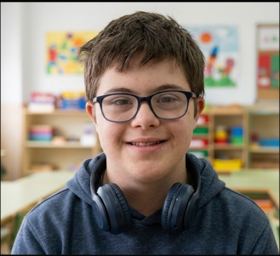
\includegraphics[width=4cm, height=4cm, keepaspectratio]{img/personas/persona3.png}%
    \vspace{0.1cm}
  }%
} \\
\hhline{|--|~|}

\cellcolor{\colorColumnaIzquierda}\textbf{Edad}
& 14 & \\
\hhline{|--|~|}

\cellcolor{\colorColumnaIzquierda}\textbf{Sexo}
& Hombre & \\
\hhline{|--|~|}

\cellcolor{\colorColumnaIzquierda}\textbf{Discapacidad}
& Visibilidad reducida & \\
\hhline{|--|~|}

\cellcolor{\colorColumnaIzquierda}\textbf{Educación}
& Alumno de Educación Especial en el Colegio Fundación Purísima Concepción	 & \\
\hline

\rowcolor{\colorEncabezado}
\multicolumn{3}{|c|}{%
  \color{\colorTextoEncabezado}\textbf{Contexto de uso}%
} \\
\hline

Cuándo
& \multicolumn{2}{Y|}{%
  \small  Cuándo	A lo largo de todo el día, tanto en horario escolar para sus encargos como por la tarde para sus aficiones%
} \\
\hline

Dónde
& \multicolumn{2}{Y|}{%
  \small En cualquier espacio del colegio (aulas, pasillos) y en su casa o lugares de ocio (como el cine)%
} \\
\hline

Tipo de ordenador
& \multicolumn{2}{Y|}{%
  \small Una tablet que pueda llevar siempre consigo, configurada con alto contraste y opciones de accesibilidad de audio%
} \\
\hline

\rowcolor{\colorEncabezado}
\multicolumn{3}{|c|}{%
  \color{\colorTextoEncabezado}\textbf{Misión}%
} \\
\hline

Objetivo
& \multicolumn{2}{Y|}{%
  \small Objetivo	Saber qué le toca hacer en cada momento del día (como sus tareas asignadas en el colegio) y poder añadir y organizar sus propias actividades de ocio (cine, escuchar música)%
} \\
\hline

Expectativas
& \multicolumn{2}{Y|}{%
  \small Espera una aplicación muy visual, con botones muy grandes debido a su reducida visión, y que le "hable" para explicarle las cosas utilizando grabaciones de voces humanas reales y amigables, ya que detesta las voces robóticas o sintéticas%
} \\
\hline

\rowcolor{\colorEncabezado}
\multicolumn{3}{|c|}{%
  \color{\colorTextoEncabezado}\textbf{Motivación}%
} \\
\hline

Urgencia
& \multicolumn{2}{Y|}{%
  \small Alta. Depende de la aplicación para estructurar su tiempo, no perderse durante el día y no olvidar las cosas que más le motivan%
} \\
\hline

Deseo
& \multicolumn{2}{Y|}{%
  \small Entusiasta pero selectivo. Le gusta usar el móvil para escuchar música y cosas de cine, pero se frustra e ignora las aplicaciones si tienen texto pequeño, poco contraste o voces artificiales que le resultan desagradables al oído%
} \\
\hline

\rowcolor{\colorEncabezado}
\multicolumn{3}{|c|}{%
  \color{\colorTextoEncabezado}\textbf{Actitud hacia la tecnología}%
} \\
\hline

Actitud
& \multicolumn{2}{Y|}{%
  \small Proactivo, como chico de su generación está familiarizado con la tecnología y entiende de forma rápida siempre que tenga una interfaz accesible y sencilla %
} \\
\hline
\end{xltabular}

\vspace{0.8cm}
\newpage
%Escenario 1
\noindent
\begin{xltabular}{\textwidth}{|p{3.5cm}|X|p{4cm}|}
\hline
\rowcolor{\colorEncabezado}
\multicolumn{3}{|c|}{%
  \color{\colorTextoEncabezado}\textbf{Escenario 1}%
} \\
\hline

Nombre persona
& Manuel García
& \multirow{4}{*}{%
  \parbox{3.8cm}{\centering
    \vspace{0.1cm}
    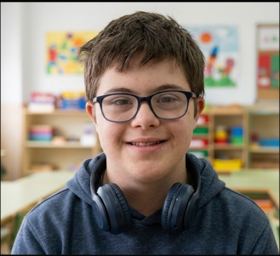
\includegraphics[width=5cm, height=5cm, keepaspectratio]{img/personas/persona3.png}%
    \vspace{0.1cm}
  }%
} \\
\cline{1-2}

Objetivo persona
& \rule{0pt}{2.5cm}Ejercer de embajador del centro enseñando los espacios a personas externas sin desorientarse ni olvidar el recorrido & \\
\hline

\rowcolor{\colorEncabezado}
\multicolumn{3}{|c|}{%
  \color{\colorTextoEncabezado}\textbf{Descripción del escenario}%
} \\
\hline

\cellcolor{\colorColumnaIzquierda}\textbf{Descripción}
& \multicolumn{2}{Y|}{%
  \small
  Es martes por la mañana. Los profesores han asignado a Manuel la tarea de "Guía de visita". Manuel saca su tablet y abre su agenda personalizada. Debido a su visión reducida, la pantalla principal está configurada con fondo negro y un pictograma amarillo muy grande y contrastado que representa una visita.
Manuel pulsa el botón grande de la tarea. Al instante, la aplicación reproduce un audio con la voz natural y cariñosa de su tutora: "¡Hola Manuel! Hoy eres nuestro embajador. Primer paso: llévalos al taller de reprografía". Manuel se siente seguro y guía a los visitantes por el pasillo. Una vez llegan al taller, Manuel saca el móvil y pulsa un botón gigante de confirmación en la pantalla para marcar el fin de ese paso.
La aplicación avanza al siguiente paso y reproduce un nuevo audio, de nuevo con voz humana, indicándole el siguiente destino de la visita. El reloj temporal accesible está oculto en su perfil para que no se ponga nervioso con el paso del tiempo. Al terminar la ruta, Manuel confirma la finalización total de la tarea y la aplicación reproduce el fragmento de su canción favorita a modo de recompensa. Manuel se siente orgulloso de haber hecho un buen trabajo por sí mismo.
%
} \\
\hline

\end{xltabular}





\vspace{0.8cm}
%Escenario 2
\noindent
\begin{xltabular}{\textwidth}{|p{3.5cm}|X|p{4cm}|}
\hline
\rowcolor{\colorEncabezado}
\multicolumn{3}{|c|}{%
  \color{\colorTextoEncabezado}\textbf{Escenario 2}%
} \\
\hline

Nombre persona
& Manuel García
& \multirow{4}{*}{%
  \parbox{3.8cm}{\centering
    \vspace{0.1cm}
    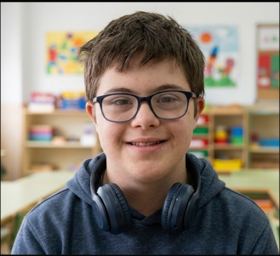
\includegraphics[width=5cm, height=5cm, keepaspectratio]{img/personas/persona3.png}%
    \vspace{0.1cm}
  }%
} \\
\cline{1-2}

Objetivo persona
& \rule{0pt}{2.5cm}Objetivo persona	Crear una tarea personal en su agenda para no olvidar el estreno de una película cuya banda sonora está deseando escuchar & \\
\hline

\rowcolor{\colorEncabezado}
\multicolumn{3}{|c|}{%
  \color{\colorTextoEncabezado}\textbf{Descripción del escenario}%
} \\
\hline

\cellcolor{\colorColumnaIzquierda}\textbf{Descripción}
& \multicolumn{2}{Y|}{%
  \small
  Es miércoles por la tarde y Manuel está en el sofá de su casa. Acaba de ver en la televisión el anuncio de una nueva película de aventuras que se estrena este viernes, y la música del tráiler le ha encantado. Sabe que quiere ir, así que coge su tablet para crear una tarea personal.
Abre la aplicación web y, navegando por su menú adaptado con letras muy grandes, selecciona la opción para añadir una nueva actividad. En lugar de tener que escribir con un teclado pequeño que apenas puede ver, Manuel utiliza un botón de grabación y dice en voz alta: "Ir al cine". El sistema reconoce la instrucción y le pide asignar una imagen. Manuel selecciona un pictograma grande de unas palomitas.
Para la descripción de la tarea, en vez de introducir texto, la aplicación le da la opción de grabar un audio descriptivo en un formato accesible para él. Manuel pulsa el botón de grabar y tararea emocionado un trozo de la canción del anuncio, añadiendo con su propia voz natural: "¡Peli nueva de aventuras!". Finalmente, configura la hora de inicio y fin para el viernes por la tarde. La tarea queda guardada en su agenda semanal y Manuel sonríe sabiendo que el viernes su tablet le avisará con su propia voz de que es la hora de ir al cine.
%
} \\
\hline

\end{xltabular}














\newpage

\subsection{Persona 4: Administrativa}

 %PERSONA 4 ADMINISTRATIVA
\noindent
\begin{xltabular}{\textwidth}{|p{3.5cm}|X|p{4cm}|}
\hline
\rowcolor{\colorEncabezado}
\multicolumn{3}{|c|}{%
  \color{\colorTextoEncabezado}\textbf{ADMINISTRATIVA}%
} \\
\hline

\cellcolor{\colorColumnaIzquierda}\textbf{Nombre}
& Carmen Ruiz
& \multirow{5}{*}{%
  \parbox{3.8cm}{\centering
    \vspace{0.1cm}
    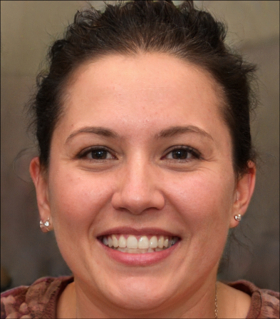
\includegraphics[width=3.8cm, height=3.8cm, keepaspectratio]{img/personas/persona4.png}%
    \vspace{0.1cm}
  }%
} \\
\hhline{|--|~|}

\cellcolor{\colorColumnaIzquierda}\textbf{Edad}
& 43 & \\
\hhline{|--|~|}

\cellcolor{\colorColumnaIzquierda}\textbf{Sexo}
& Mujer & \\
\hhline{|--|~|}

\cellcolor{\colorColumnaIzquierda}\textbf{Discapacidad}
& No tiene & \\
\hhline{|--|~|}

\cellcolor{\colorColumnaIzquierda}\textbf{Educación}
&Personal de Administración y Servicios (PAS) / Técnico en Gestión Administrativa	 & \\
\hline

\rowcolor{\colorEncabezado}
\multicolumn{3}{|c|}{%
  \color{\colorTextoEncabezado}\textbf{Contexto de uso}%
} \\
\hline

Cuándo
& \multicolumn{2}{Y|}{%
  \small  Cuándo	Principalmente al inicio del curso escolar (o de la implantación del sistema) para realizar la carga de datos masiva, y de forma esporádica durante el curso para gestionar nuevas altas, bajas o reasignaciones.%
} \\
\hline

Dónde
& \multicolumn{2}{Y|}{%
  \small En las instalaciones del Colegio de Educación Especial de la Fundación Purísima Concepción, desde un despacho o secretaría.%
} \\
\hline

Tipo de ordenador
& \multicolumn{2}{Y|}{%
  \small Tipo de ordenador	Ordenador de sobremesa del centro educativo o portátil de trabajo.%
} \\
\hline

\rowcolor{\colorEncabezado}
\multicolumn{3}{|c|}{%
  \color{\colorTextoEncabezado}\textbf{Misión}%
} \\
\hline

Objetivo
& \multicolumn{2}{Y|}{%
  \small Crear las cuentas de acceso de todos los usuarios de la plataforma: unos 100-150 estudiantes, además de profesores y tutores. Su labor principal es establecer las relaciones en el sistema, asignando qué estudiantes corresponden a cada profesor y a cada familiar para que ellos gestionen el resto.%
} \\
\hline

Expectativas
& \multicolumn{2}{Y|}{%
  \small Espera encontrar un panel de administración robusto, rápido e intuitivo que le permita gestionar este volumen de usuarios de forma eficiente y sin errores, garantizando que los profesores y estudiantes puedan acceder sin problemas para personalizar sus agendas%
} \\
\hline

\rowcolor{\colorEncabezado}
\multicolumn{3}{|c|}{%
  \color{\colorTextoEncabezado}\textbf{Motivación}%
} \\
\hline

Urgencia
& \multicolumn{2}{Y|}{%
  \small Media. En el colegio tienen una agenda física ya hecha desde hace unos años, pero una aplicación web facilita la logística y sería más amigable con el medio ambiente%
} \\
\hline

Deseo
& \multicolumn{2}{Y|}{%
  \small Desea que la fase de implantación tecnológica sea un éxito y estructurar correctamente la base de usuarios para facilitar la autonomía de los alumnos del Programa de Transición a la Vida Adulta (PTVAL) y el trabajo de los docentes%
} \\
\hline

\rowcolor{\colorEncabezado}
\multicolumn{3}{|c|}{%
  \color{\colorTextoEncabezado}\textbf{Actitud hacia la tecnología}%
} \\
\hline

Actitud
& \multicolumn{2}{Y|}{%
  \small Pragmática y centrada en la eficiencia. Al tener que manejar el registro de unas 100-150 personas, valora por encima de todo las interfaces claras, sin pasos innecesarios, que no le hagan perder tiempo y le eviten incidencias técnicas de acceso con los padres y profesores %
} \\
\hline
\end{xltabular}

\vspace{0.8cm}
\newpage
%Escenario 1
\noindent
\begin{xltabular}{\textwidth}{|p{3.5cm}|X|p{4cm}|}
\hline
\rowcolor{\colorEncabezado}
\multicolumn{3}{|c|}{%
  \color{\colorTextoEncabezado}\textbf{Escenario 1}%
} \\
\hline

Nombre persona
& Carmen Ruiz
& \multirow{4}{*}{%
  \parbox{3.8cm}{\centering
    \vspace{0.1cm}
    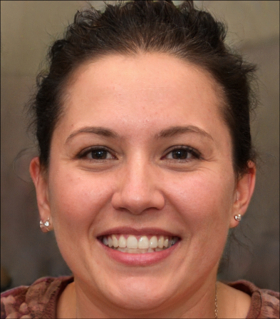
\includegraphics[width=5.5cm, height=5.5cm, keepaspectratio]{img/personas/persona4.png}%
    \vspace{0.1cm}
  }%
} \\
\cline{1-2}

Objetivo persona
& \rule{0pt}{2.5cm} Registrar las cuentas de los estudiantes, profesores y familiares, y vincular a cada estudiante con su tutor y su familia correspondiente para que puedan empezar a usar la aplicación web& \\
\hline

\rowcolor{\colorEncabezado}
\multicolumn{3}{|c|}{%
  \color{\colorTextoEncabezado}\textbf{Descripción del escenario}%
} \\
\hline

\cellcolor{\colorColumnaIzquierda}\textbf{Descripción}
& \multicolumn{2}{Y|}{%
  \small
  Es la primera semana de septiembre en el Colegio de Educación Especial Fundación Purísima Concepción. Carmen, sentada frente al ordenador de secretaría, recibe el listado definitivo de matriculaciones para el nuevo curso. Este año, el centro ha decidido dar el salto y sustituir la tradicional agenda física por la nueva aplicación web, una decisión que a Carmen le motiva porque facilitará la logística diaria y es mucho más respetuosa con el medio ambiente.
Sabe que tiene que registrar a algo más de 100 alumnos, además de a sus profesores y familiares, por lo que entra a la plataforma con su cuenta de administrador con la intención de dejarlo todo listo antes del primer día de clases. Navega al panel de gestión y comienza a introducir los datos. La aplicación le permite ir creando las cuentas de los estudiantes y, en el mismo flujo de trabajo, asignarles quién será su profesor y qué familiares tendrán acceso a su perfil.
A mitad del proceso, el teléfono de secretaría suena; es un padre haciendo una consulta administrativa. Carmen atiende la llamada y, al volver a la pantalla, agradece que el sistema sea claro y le permita retomar el registro exactamente donde lo dejó sin perder la información. Una vez finalizada la carga de todos los usuarios, Carmen pulsa un botón para enviar de forma masiva las credenciales de acceso a los correos de los profesores y los padres. Respira aliviada al ver que el proceso ha sido fluido y sin bloqueos técnicos; ahora el sistema está preparado para que cada familia y profesor entre a personalizar las agendas de sus respectivos alumnos%

} \\
\hline

\end{xltabular}




\newpage

\subsection{Persona 5: Estudiante con discapacidad intelectual}

 %PERSONA 5 ESTUDIANTE CON DISCAPACIDAD INTELECTUAL
\noindent
\begin{xltabular}{\textwidth}{|p{3.5cm}|X|p{4cm}|}
\hline
\rowcolor{\colorEncabezado}
\multicolumn{3}{|c|}{%
  \color{\colorTextoEncabezado}\textbf{ESTUDIANTE CON DISCAPACIDAD INTELECTUAL}%
} \\
\hline

\cellcolor{\colorColumnaIzquierda}\textbf{Nombre}
& Daniela Martín
& \multirow{5}{*}{%
  \parbox{3.8cm}{\centering
    \vspace{0.1cm}
    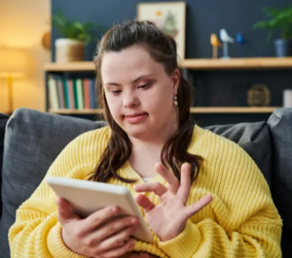
\includegraphics[width=3.8cm, height=3.8cm, keepaspectratio]{img/personas/persona5.png}%
    \vspace{0.1cm}
  }%
} \\
\hhline{|--|~|}

\cellcolor{\colorColumnaIzquierda}\textbf{Edad}
& 19 & \\
\hhline{|--|~|}

\cellcolor{\colorColumnaIzquierda}\textbf{Sexo}
& Mujer & \\
\hhline{|--|~|}

\cellcolor{\colorColumnaIzquierda}\textbf{Discapacidad}
& Discapacidad Intelectual & \\
\hhline{|--|~|}

\cellcolor{\colorColumnaIzquierda}\textbf{Educación}
&	Estudiante del Programa de Transición a la Vida Adulta (PTVAL) & \\
\hline

\rowcolor{\colorEncabezado}
\multicolumn{3}{|c|}{%
  \color{\colorTextoEncabezado}\textbf{Contexto de uso}%
} \\
\hline

Cuándo
& \multicolumn{2}{Y|}{%
  \small Utiliza la aplicación a lo largo del día para consultar las actividades que tiene programadas, tanto en el centro, al comenzar la jornada, antes de realizar una tarea o al terminarla, como en casa, para consultar sus actividades personales y las tareas programadas  %
} \\
\hline

Dónde
& \multicolumn{2}{Y|}{%
  \small En el centro educativo y en casa%
} \\
\hline

Tipo de ordenador
& \multicolumn{2}{Y|}{%
  \small Teléfono móvil o Tablet%
} \\
\hline

\rowcolor{\colorEncabezado}
\multicolumn{3}{|c|}{%
  \color{\colorTextoEncabezado}\textbf{Misión}%
} \\
\hline

Objetivo
& \multicolumn{2}{Y|}{%
  \small Consultar y seguir su agenda personalizada para saber qué actividades tiene programadas, cuándo debe realizarlas, qué pasos debe seguir y cuánto durará cada actividad, tanto en el centro como en su vida cotidiana%
} \\
\hline

Expectativas
& \multicolumn{2}{Y|}{%
  \small Espera encontrar una agenda sencilla, clara y adaptada a sus necesidades, que le permita identificar fácilmente cada actividad mediante imágenes, saber cuándo comienza y termina y recibir avisos que le ayuden a anticipar los cambios. También espera poder consultar instrucciones accesibles mediante texto, audio, o secuencias de imágenes cuando necesite ayuda para realizar una tarea%
} \\
\hline

\rowcolor{\colorEncabezado}
\multicolumn{3}{|c|}{%
  \color{\colorTextoEncabezado}\textbf{Motivación}%
} \\
\hline

Urgencia
& \multicolumn{2}{Y|}{%
  \small Urgencia	Necesita consultar la agenda durante el día, especialmente cuando comienza una actividad, cuando termina una tarea o cuando necesita saber qué tiene que hacer a continuación%
} \\
\hline

Deseo
& \multicolumn{2}{Y|}{%
  \small Quiere saber con antelación qué va a hacer y cuánto tiempo tiene para cada actividad, para sentirse seguro y poder realizar sus tareas con mayor autonomía, reduciendo la necesidad de preguntar continuamente a otras personas%
} \\
\hline

\rowcolor{\colorEncabezado}
\multicolumn{3}{|c|}{%
  \color{\colorTextoEncabezado}\textbf{Actitud hacia la tecnología}%
} \\
\hline

Actitud
& \multicolumn{2}{Y|}{%
  \small  Precavida, ya que requiere aplicaciones sencillas que tengan interfaces intuitivas, con pocos elementos, imágenes, botones y texto grandes %
} \\
\hline
\end{xltabular}

\vspace{0.8cm}
\newpage
%Escenario 1
\noindent
\begin{xltabular}{\textwidth}{|p{3.5cm}|X|p{4cm}|}
\hline
\rowcolor{\colorEncabezado}
\multicolumn{3}{|c|}{%
  \color{\colorTextoEncabezado}\textbf{Escenario 1}%
} \\
\hline

Nombre persona
& Daniela Martín
& \multirow{4}{*}{%
  \parbox{3.8cm}{\centering
    \vspace{0.1cm}
    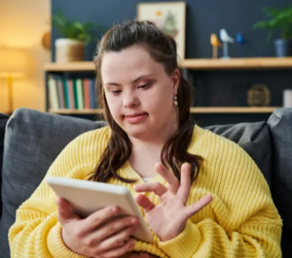
\includegraphics[width=4.5cm, height=4.5cm, keepaspectratio]{img/personas/persona5.png}%
    \vspace{0.1cm}
  }%
} \\
\cline{1-2}

Objetivo persona
& \rule{0pt}{2.5cm} Saber qué actividades tiene programadas, cuándo debe realizarlas y qué pasos debe seguir para poder realizarlas de forma autónoma y con seguridad en el centro& \\
\hline

\rowcolor{\colorEncabezado}
\multicolumn{3}{|c|}{%
  \color{\colorTextoEncabezado}\textbf{Descripción del escenario}%
} \\
\hline

\cellcolor{\colorColumnaIzquierda}\textbf{Descripción}
& \multicolumn{2}{Y|}{%
  \small
  Daniela comienza una mañana de su jornada en el centro y consulta su agenda para conocer las actividades programadas para ese día. Entre ellas encuentra una tarea de reprografía añadida previamente por el profesor, donde puede visualizar el nombre de la actividad, la imagen asociada y el horario en el que debe realizarla.
Cuando llega la hora indicada, la aplicación la avisa de que debe comenzar. Daniela consulta la tarea y visualiza una secuencia de imágenes que le indica los pasos que debe seguir. Primero debe recoger un material en un aula, después llevarlo al taller de reprografía para realizar las copias y finalmente volver al aula para repartir el material.
Daniela confirma el inicio de la tarea y comienza a realizarla. Mientras trabaja, puede consultar el tiempo restante mediante el reloj temporal, que tiene configurado en su perfil. Las imágenes le indican qué debe hacer a continuación, lo que le permite realizar la actividad con mayor autonomía. Además, puede ir marcando las tareas que ha ido realizando conforme va avanzando en la actividad.
Una vez finalizada la actividad, Daniela la marca como completada y la aplicación actualiza automáticamente su agenda, mostrando la siguiente actividad programada para que pueda continuar su jornada sin depender de las indicaciones constantes del tutor
%

} \\
\hline

\end{xltabular}




\vspace{0.8cm}
\newpage
%Escenario 2
\noindent
\begin{xltabular}{\textwidth}{|p{3.5cm}|X|p{4cm}|}
\hline
\rowcolor{\colorEncabezado}
\multicolumn{3}{|c|}{%
  \color{\colorTextoEncabezado}\textbf{Escenario 2}%
} \\
\hline

Nombre persona
& Daniela Martín
& \multirow{4}{*}{%
  \parbox{3.8cm}{\centering
    \vspace{0.1cm}
    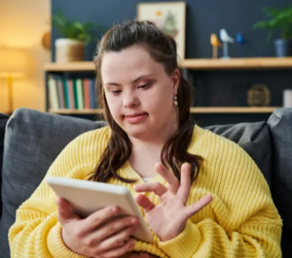
\includegraphics[width=4.5cm, height=4.5cm, keepaspectratio]{img/personas/persona5.png}%
    \vspace{0.1cm}
  }%
} \\
\cline{1-2}

Objetivo persona
& \rule{0pt}{2.5cm} Saber qué actividades tiene programadas, cuándo debe realizarlas y qué pasos debe seguir para poder realizarlas de forma autónoma y con seguridad en casa& \\
\hline

\rowcolor{\colorEncabezado}
\multicolumn{3}{|c|}{%
  \color{\colorTextoEncabezado}\textbf{Descripción del escenario}%
} \\
\hline

\cellcolor{\colorColumnaIzquierda}\textbf{Descripción}
& \multicolumn{2}{Y|}{%
  \small
  Daniela ha finalizado su jornada en el centro y al volver a casa vuelve a consultar su agenda para ver las actividades personales que ella misma o sus padres han añadido, como hacer los deberes, regar las plantas o una quedada con amigos. 
Ese día, Daniela tiene programada a las cinco una quedada con sus amigos en el parque. Sin embargo, cuando llega la hora de realizarla, comienza a llover y Daniela recibe una notificación indicando que la actividad ha sido cancelada por sus padres debido a la lluvia. La aplicación actualiza automáticamente su agenda y le muestra una propuesta alternativa para realizar en casa, como dibujar.
Una vez finalizada la actividad alternativa, Daniela confirma que la ha completado y la aplicación le permite evaluar si le ha gustado. Así, la aplicación registra sus preferencias para ofrecer actividades adaptadas a sus gustos en futuras ocasiones

%

} \\
\hline

\end{xltabular}
\newpage
\section{Visión del Producto: Elevator Pitch}

\vspace{0.3cm}

\begingroup
\renewcommand{\arraystretch}{1.6}
\setlength{\arrayrulewidth}{0.8pt}

\begin{xltabular}{\linewidth}{>{\columncolor{azulclaro}\bfseries\sffamily\color{black}} p{3.5cm} X}
    \rowcolor{azulPastelApagado}
    \multicolumn{2}{c}{\Large\bfseries\sffamily ELEVATOR PITCH — Proyecto: Doble Agenda} \\[4pt] \hline\hline
    
    PARA & Para estudiantes con discapacidad intelectual, especialmente aquellos del Programa de Transición a la Vida Adulta (\textbf{PTVAL}), y sus tutores, tanto del ámbito educativo como familiar. \\ \hline
    
    QUÉ & Necesitan una herramienta accesible y personalizada que les ayude a organizar su tiempo, comprender las actividades que deben realizar y llevarlas a cabo de forma autónoma. \\ \hline
    
    \rowcolor{verdeApagado!30}
    EL PRODUCTO & {\Large \bfseries Doble Agenda} \\ \hline
    
    ES UN & Aplicación web de una agenda personal accesible, orientada a la planificación y el seguimiento de actividades. \\ \hline
    
    QUE PROPORCIONA & Proporciona una agenda personalizada con tareas organizadas por horarios, avisos temporales e instrucciones adaptadas mediante texto, imágenes, audio o vídeo.\\[3pt]
    Permite a los estudiantes indicar el inicio y finalización de las actividades y marcar tareas realizadadas, mientras que los tutores pueden crear/asignar tareas, configurar preferencias y consultar el progreso. \\ \hline
\end{xltabular}
\endgroup

\section{Plan de Entregas}

\subsection{Breve descripción del alcance del sistema}
El proyecto consiste en el diseño, planificación y desarrollo de una aplicación web acerca de una agenda personalizada, orientada a facilitar la organización, autonomía y estructuración del tiempo a estudiantes con discapacidad intelectual, especialmente del Programa de Transición a la Vida Adulta (PTVAL).

Algunos de los objetivos principales son:

\begin{itemize}
    \item \textbf{Gestión de Tareas Escolares y Específicas:} Permitir la asignación y seguimiento de tareas propias del centro educativo (como reprografía, comedor, menú mensual, guías de visita) por parte del profesorado y de los estudiantes..
    \item \textbf{Creación y Gestión de actividades Personales:} Dar autonomía a los estudiantes y padres o madres para crear actividades cotidianas con horas de inicio/fin, imágenes, y formatos accesibles (texto, audio, vídeo o secuencias de pasos).
    \item \textbf{Adaptabilidad y Accesibilidad Total:} Configurar perfiles personalizados que ajusten colores, tipos y tamaños de letra, disposición de menús y botones.
    \item \textbf{Roles Definidos:} Estructurar los permisos y funcionalidades para Administradores, Profesores/Tutores y Estudiantes.
\end{itemize}

\subsection{Listado Inicial de HU}

\begin{xltabular}{\textwidth}{p{1.8cm} X p{1.3cm} p{1.1cm}}
\toprule
\rowcolor{azulPastelApagado}
\textbf{Ident.} & \textbf{Título} & \textbf{Estim.} & \textbf{Prio.} \\
\midrule
\endhead

\bottomrule
\endfoot

\rowcolors{2}{azulclaro}{white}
HU-F1 & Como Familia quiero iniciar sesión en la aplicación para acceder a la funcionalidad de esta. & 3 & 2 \\
HU-F2 & Como Familia quiero seleccionar uno de mis hijos para acceder a su perfil. & 1 & 2 \\
HU-F3 & Como Familia quiero consultar el perfil de un hijo para ver su configuración. & 1 & 3 \\
HU-F4 & Como Familia quiero cambiar la configuración de un hijo para hacer la aplicación más accesible para él/ella. & 1 & 3 \\
HU-F5 & Como Familia quiero comprobar la agenda de un hijo para ver sus actividades planeadas . & 2 & 2 \\
HU-F6 & Como Familia quiero consultar los detalles específicos de una actividad que tiene mi hijo para conocer los detalles de esta. & 2 & 3 \\
HU-F7 & Como Familia quiero crear una actividad con pasos o sin pasos, para un hijo para que pueda tenerla presente y pueda realizarla por su cuenta. & 5 & 2 \\
HU-F8 & Como Familia quiero editar una actividad que le cree a mi hijo para corregir o añadir detalles de esta. & 5 & 3 \\
HU-F9 & Como Familia quiero borrar una actividad que le cree a mi hijo para que no la realice. & 5 & 3 \\
HU-P1 & Como profesor/a, quiero iniciar sesión en la aplicación para consultar la agenda escolar. & 3 & 1 \\
HU-P2 & Como profesor/a, quiero consultar las actividades programadas y sus detalles para conocer la información necesaria sobre cada actividad. & 2 & 1 \\
HU-P3 & Como profesor/a, quiero crear actividades con pasos o sin pasos, para mantener actualizada la planificación escolar según las necesidades del alumnado.~ & 5 & 1 \\
HU-P4 & Como profesor/a, quiero cancelar actividades para mantener actualizada la planificación escolar según las necesidades del alumnado.~ & 5 & 2 \\
HU-P5 & Como profesor/a, quiero editar actividades para mantener actualizada la planificación escolar según las necesidades del alumnado.~ & 5 & 3 \\
HU-P6 & Como profesor/a, quiero asignar una actividad a un estudiante o grupo para adaptar la planificación a sus necesidades educativas.~ & 3 & 1 \\
HU-P7 & Como profesor/a, quiero consultar qué estudiantes participan en una actividad para conocer quiénes deben realizarla y organizar su desarrollo.~ & 2 & 3 \\
HU-P8 & Como profesor/a, quiero consultar qué estudiantes han comenzado o completado una actividad para realizar un seguimiento individual de su progreso.~ & 8 & 4 \\
HU-P9 & Como profesor/a, quiero marcar una actividad como realizada para mantener actualizado el calendario y registrar las actividades que ya se han llevado a cabo.~ & 2 & 3 \\
HU-P10 & Como profesor/a, quiero consultar la información relevante de un estudiante. & 3 & 2 \\
HU-E1 & Como estudiante, quiero iniciar sesión en la aplicación en función de mis necesidades de accesibilidad, para acceder a mi agenda y a mis actividades personales.~ & 3 & 1 \\
HU-E2 & Como estudiante, quiero consultar mi agenda personalizada, para saber qué actividades tengo programadas durante el día. & 3 & 1 \\
HU-E3 & Como estudiante, quiero consultar la información de una actividad para comprender fácilmente qué tengo que hacer.~ & 3 & 1 \\
HU-E4 & Como estudiante, quiero consultar las actividades de los próximos días, para organizarme y saber qué tengo programado durante la semana.~ & 3 & 1 \\
HU-E5 & Como estudiante, quiero añadir actividades personales a mi agenda, para organizar mis actividades de forma autónoma.~ & 5 & 3 \\
HU-E7 & Como estudiante, quiero marcar los pasos de una actividad conforme los voy realizando, para saber qué pasos he completado y cuál debo realizar a continuación. & 2 & 3 \\
HU-E8 & Como estudiante, quiero consultar el tiempo restante de una actividad, para saber cuánto tiempo tengo para realizarla.~ & 2 & 4 \\
HU-E9 & Como estudiante, quiero confirmar el inicio de una actividad, para registrar su inicio y llevar un seguimiento de mi progreso.~ & 1 & 4 \\
HU-E10 & Como estudiante, quiero confirmar la finalización de una actividad, para registrar su finalización y saber qué actividad debo realizar a continuación.~ & 1 & 3 \\
HU-E12 & Como estudiante, quiero recibir una sugerencia de actividad alternativa cuando se cancele una actividad programada, para saber qué puedo hacer en su lugar y mantener organizada mi rutina.~ & 21 & 5 \\
HU-E13 & Como estudiante, quiero valorar una actividad realizada, para que la aplicación pueda tener en cuenta mis preferencias en futuras sugerencias.~ & 5 & 5 \\
HU-E14 & Como estudiante, quiero adaptar las preferencias de visualización de mi agenda a mis necesidades, para consultar las actividades de una forma que me resulte cómoda y comprensible.~ & 8 & 2 \\
HUT-A0 & Como administrador técnico de nuestra empresa quiero montar infraestructura de la aplicación para que mis usuarios puedan utilizarla.~ & 2 & 1 \\
HU-A1 & Como administrador quiero crear un usuario estudiante para que cierto estudiante pueda usar la aplicación.~ & 2 & 1 \\
HU-A2 & Como administrador quiero crear usuarios profesor y familia para que cierto profesor y familiar pueda usar la aplicación & 1 & 1 \\
HU-A3 & Como administrador quiero eliminar usuarios para cuando dejen de estar en la institución y ahorrar almacenamiento.~ & 1 & 3 \\
HU-A4 & Como administrador quiero asignar un estudiante /profesor a un grupo de clase para que yo y los usuarios trabajen con interfaces con menos opciones & 2 & 2 \\
HU-A5 & Como administrador quiero asignar un profesor a un estudiante para que el profesor pueda interactuar con la agenda del estudiante & 2 & 1 \\
HU-A6 & Como administrador quiero asignar un padre/madre/tutor a un estudiante para que el padre pueda/madre/tutor pueda interactuar con la agenda del estudiante.~ & 2 & 2 \\
\end{xltabular}



\subsection{Cálculo de la velocidad del equipo.}
Partimos de un equipo de desarrollo formado por 5 programadores que van a dedicar un 50\% de su tiempo de trabajo al proyecto (debido a otras asignaturas). La duración de cada una de las iteraciones que vamos a realizar en el proyecto van a ser de 3 semanas. La estimación realizada del esfuerzo de cada una de las historias de usuario se ha expresado en días ideales de programación. En nuestro entorno de trabajo estimamos que un día ideal de programación se va a corresponder con 2 a 3 días reales de trabajo.

La duración de una iteración va a ser:
\begin{center}
1 Iteración = 3 semanas = 15 Días reales
\end{center}

\begin{itemize}
    \item 1ª iteracion $\rightarrow$ 33  
    \item 2ª iteracion $\rightarrow$ 33
    \item 3ª iteracion $\rightarrow$ 31
    \item 4ª iteracion $\rightarrow$ 13
    \item 5ª iteracion $\rightarrow$ 21
\end{itemize}

La Velocidad del equipo de desarrollo medido en punto de historia es:
\begin{center}
5 Programadores * 15 = 75 días reales por iteración: de 25 a 38 PH por iteración. Se ha decidido usar 33 Puntos de historia como la velocidad estimada del equipo.
\end{center}

\subsection{Descripción de las entregas.}

Esfuerzo total del proyecto =  PH 

Velocidad del equipo = 33 PH (por iteración) 

En base al esfuerzo necesario y la velocidad estimada del equipo, para el desarrollo del proyecto se van a realizar una entregas de tres iteraciones cada  una de ellas. 

El desarrollo del producto empieza el 22 de Octubre y el plan de entregas es el siguiente:

\begin{description}[font=\normalfont, style=multiline, leftmargin=3.2cm]
    \item[{Iteración 1:}] Hasta el 11 de Noviembre. El objetivo es crear una aplicación funcional que permita registrar estudiantes y profesores, que estos inicien sesión, crear y asignar tareas y que los perfiles de usuario puedan visualizar la agenda con las tareas a un nivel básico.
    \item[{Iteración 2:}] Hasta 2 de Diciembre. El objetivo es añadir el perfil de la familia, completar el de administrador y ampliar funcionalidades básicas.
    \item[{Iteración 3:}] Hasta 21 de Diciembre. El objetivo es implementar toda la personalización del usuario y lo referente a la accesibilidad.
    \item[{Iteración 4:}] Hasta finales de Diciembre. Buscaremos implementar funcionalidades de calidad de vida de la aplicación.
    \item[{Iteración 5:}] Hasta finales de Enero. Implementaremos un sistema de actividades optativas.
\end{description}


\section{Backlog del Producto}

\begin{xltabular}{\textwidth}{|p{2.2cm}|X|p{1.4cm}|p{1.7cm}|p{1.5cm}|}
\hline
\rowcolor{azulPastelApagado}
\textbf{Ident.} & \textbf{Título} & \textbf{Estim.} & \textbf{Iteración} & \textbf{Entrega} \\ \hline
\endhead

\hline
\endfoot

\rowcolors{2}{azulclaro}{white}
HU-P1 & Como profesor/a, quiero iniciar sesión en la aplicación para consultar la agenda escolar. & 3 & 1 & 1 \\ \hline
HU-P2 & Como profesor/a, quiero consultar las actividades programadas y sus detalles para conocer la información necesaria sobre cada actividad. & 2 & 1 & 1 \\ \hline
HU-P3 & Como profesor/a, quiero crear actividades para mantener actualizada la planificación escolar según las necesidades del alumnado. & 5 & 1 & 1 \\ \hline
HU-P6 & Como profesor/a, quiero asignar una actividad a un estudiante o grupo para adaptar la planificación a sus necesidades educativas. & 3 & 1 & 1 \\ \hline
HU-E1 & Como estudiante, quiero iniciar sesión en la aplicación, para acceder a mi agenda y a mis actividades personales. & 3 & 1 & 1 \\ \hline
HU-E2 & Como estudiante, quiero consultar mi agenda personalizada, para saber qué actividades tengo programadas durante el día. & 3 & 1 & 1 \\ \hline
HU-E3 & Como estudiante, quiero consultar la información de una actividad para comprender fácilmente qué tengo que hacer. & 3 & 1 & 1 \\ \hline
HU-E4 & Como estudiante, quiero consultar las actividades de los próximos días, para organizarme y saber qué tengo programado durante la semana. & 2 & 1 & 1 \\ \hline
HUT-A0 & Como administrador quiero montar infraestructura de la aplicación para que mis usuarios puedan utilizarla. & 2 & 1 & 1 \\ \hline
HU-A1 & Como administrador quiero crear un usuario estudiante para que cierto estudiante pueda usar la aplicación. & 2 & 1 & 1 \\ \hline
HU-A2 & Como administrador quiero crear usuarios profesor y familia para que cierto profesor y familiar pueda usar la aplicación & 1 & 1 & 1 \\ \hline
HU-A4 & Como administrador quiero asignar un estudiante /profesor a un grupo de clase para que yo y los usuarios trabajen con interfaces con menos opciones & 2 & 1 & 1 \\ \hline
HU-A5 & Como administrador quiero asignar un profesor a un estudiante para que el profesor pueda interactuar con la agenda del estudiante & 2 & 1 & 1 \\ \hline
HU-F1 & Como Familia quiero iniciar sesión en la aplicación para acceder a la funcionalidad de esta. & 3 & 2 & 2 \\ \hline
HU-F2 & Como Familia quiero seleccionar uno de mis hijos para acceder a su perfil. & 1 & 2 & 2 \\ \hline
HU-F5 & Como Familia quiero comprobar la agenda de un hijo para ver sus actividads planeadas. & 2 & 2 & 2 \\ \hline
HU-F7 & Como Familia quiero crear una actividad para un hijo para que pueda tenerla presente y pueda realizarla por su cuenta. & 5 & 2 & 2 \\ \hline
HU-P4 & Como profesor/a, quiero cancelar actividades para mantener actualizada la planificación escolar según las necesidades del alumnado. & 5 & 2 & 2\\ \hline
HU-P7 & Como profesor/a, quiero consultar qué estudiantes participan en una actividad para conocer quiénes deben realizarla y organizar su desarrollo. & 2 & 2 & 2 \\ \hline
HU-P10 & Como profesor/a, quiero consultar la información relevante de un estudiante para adaptar las actividades a sus necesidades y facilitar su participación y aprendizaje. & 3 & 2 & 2 \\ \hline
HU-E7 & Como estudiante, quiero marcar los pasos de una actividad conforme los voy realizando, para saber qué pasos he completado y cuál debo realizar a continuación. & 2 & 2 & 2 \\ \hline
HU-E14 & Como estudiante, quiero adaptar las preferencias de visualización de mi agenda a mis necesidades, para consultar las actividades de una forma que me resulte cómoda y comprensible. & 8 & 2 & 2 \\ \hline
HU-A6 & Como administrador quiero asignar un padre/madre/tutor a un estudiante para que el padre pueda/madre/tutor pueda interactuar con la agenda del estudiante. & 2 & 2 & 2 \\ \hline
HU-F3 & Como Familia quiero consultar el perfil de un hijo para ver su configuración. & 1 & 3 & 3 \\ \hline
HU-F4 & Como Familia quiero cambiar la configuración de un hijo para hacer la aplicación más accesible para él/ella. & 1 & 3 & 3 \\ \hline
HU-F6 & Como Familia quiero consultar los detalles específicos de una actividad que tiene mi hijo para conocer los detalles de esta. & 2 & 3 & 3 \\ \hline
HU-F8 & Como Familia quiero editar una actividad que le cree a mi hijo para corregir o añadir detalles de esta. & 5 & 3 & 3 \\ \hline
HU-F9 & Como Familia quiero borrar una actividad que le cree a mi hijo para que no la realice. & 5 & 3 & 3 \\ \hline
HU-P5 & Como profesor/a, quiero editar actividades para mantener actualizada la planificación escolar según las necesidades del alumnado. & 5 & 3 & 3 \\ \hline
HU-P9 & Como profesor/a, quiero marcar una actividad como realizada para mantener actualizado el calendario y registrar las actividades que ya se han llevado a cabo. & 2 & 3 & 3 \\ \hline
HU-E5 & Como estudiante, quiero añadir actividades personales a mi agenda, para organizar mis actividads y actividades cotidianas en casa de forma autónoma. & 5 & 3 & 3 \\ \hline
HU-E8 & Como estudiante, quiero consultar el tiempo restante de una actividad, para saber cuánto tiempo tengo para realizarla. & 2 & 3 & 3 \\ \hline
HU-E9 & Como estudiante, quiero confirmar el inicio de una actividad, para registrar su inicio y llevar un seguimiento de mi progreso. & 1 & 3 & 3 \\ \hline
HU-E10 & Como estudiante, quiero confirmar la finalización de una actividad, para registrar su finalización y saber qué actividad debo realizar a continuación. & 1 & 3 & 3 \\ \hline
HU-A3 & Como administrador quiero eliminar usuarios para cuando dejen de estar en la institución y ahorrar almacenamiento. & 1 & 3 & 3 \\ \hline
HU-P8 & Como profesor/a, quiero consultar qué estudiantes han comenzado o completado una actividad para realizar un seguimiento individual de su progreso. & 8 & 4 & 4 \\ \hline
HU-E6 & Como estudiante, quiero recibir avisos cuando llegue la hora de realizar una actividad, para saber cuándo debo comenzar. & 8 & 4 & 4 \\ \hline
HU-E11 & Como estudiante, quiero recibir un aviso cuando se cancele una actividad de mi agenda, para saber que ya no tengo que realizarla. & 3 & 4 & 4 \\ \hline
HU-F10 & Como Familia quiero abrir un canal de comunicación en la aplicación con mi hijo para poder comunicarme con él & 21 & 5 & 5 \\ \hline
HU-E12 & Como estudiante, quiero recibir una sugerencia de actividad alternativa cuando se cancele una actividad programada, para saber qué puedo hacer en su lugar y mantener organizada mi rutina. & 21 & 5 & 5 \\ \hline
HU-E13 & Como estudiante, quiero valorar una actividad realizada, para que la aplicación pueda tener en cuenta mis preferencias en futuras sugerencias. & 5 & 5 & 5 \\ \hline
HU-E15 & Como estudiante, quiero enviar mensajes a través de un chat accesible, para solicitar ayuda o resolver dudas mientras realizo mis actividades. & 21 & 5 & 5 \\ \hline
HU-E16 & Como estudiante, quiero recibir mensajes a través de un chat accesible, para recibir indicaciones, en caso de necesitarlo, mientras realizo mis actividades. & 21 & 5 & 5 \\ \hline
\end{xltabular}
\noindent\textit{Nota sobre el alcance de las iteraciones:} El desarrollo principal del
 proyecto abarca estrictamente las **Iteraciones 1, 2 y 3**. Las Historias de Usuario asignadas 
 a la **Iteración 4** únicamente se abordarán si se dispone de tiempo suficiente tras completar las iteraciones principales en la entrega final. Por su parte, las funcionalidades marcadas en la **Iteración 5** quedan explícitamente fuera del alcance comprometido para este proyecto debido a su elevada complejidad.
\vspace{0.4cm}
\subsection{Tarjetas de la HU (Primera Iteración)}

\begin{table}[H]
\centering
\rowcolors{1}{white}{white}
\begin{tabularx}{\textwidth}{|X|X|X|}
\hline
\rowcolor{azulclaro}
\multicolumn{1}{|l|}{\textbf{Identificador:} HU-P1} & \multicolumn{2}{l|}{\textbf{Iniciar sesión}} \\ \hline
\multicolumn{3}{|p{\dimexpr\textwidth-2\tabcolsep-2\arrayrulewidth}|}{\textbf{Descripción:} Como profesor/a, quiero iniciar sesión en la aplicación para consultar la agenda escolar.} \\ \hline
\rowcolor{white}
\textbf{Estimación: 3} & \textbf{Prioridad: 1} & \textbf{Entrega: 1} \\ \hline
\multicolumn{3}{|p{\dimexpr\textwidth-2\tabcolsep-2\arrayrulewidth}|}{%
\textbf{Pruebas de aceptación:}
\begin{itemize}[leftmargin=1.5em, itemsep=2pt, topsep=3pt]
    \item En caso de introducir unas credenciales válidas, el sistema permite al profesor/a iniciar sesión y acceder a la aplicación.
    \item En caso de introducir un correo electrónico o una contraseña incorrectos, el sistema avisa de que las credenciales no son válidas y deniega el acceso.
    \item En caso de intentar iniciar sesión sin introducir alguno de los campos obligatorios, el sistema avisa de que faltan datos y deniega el acceso.
    \item En caso de intentar iniciar sesión con una cuenta que no está registrada en el sistema, el sistema avisa de que las credenciales no son válidas y deniega el acceso.
\end{itemize}
} \\ \hline
\multicolumn{3}{|p{\dimexpr\textwidth-2\tabcolsep-2\arrayrulewidth}|}{\textbf{Observaciones:} Requiere implementar un sistema de autenticación de usuarios.} \\ \hline
\end{tabularx}
\end{table}

\vspace{0.4cm}

\begin{table}[H]
\centering
\rowcolors{1}{white}{white}
\begin{tabularx}{\textwidth}{|X|X|X|}
\hline
\rowcolor{azulclaro}
\multicolumn{1}{|l|}{\textbf{Identificador:} HU-P2} & \multicolumn{2}{l|}{\textbf{Consultar actividades programadas y sus detalles}} \\ \hline
\multicolumn{3}{|p{\dimexpr\textwidth-2\tabcolsep-2\arrayrulewidth}|}{\textbf{Descripción:} Como profesor/a, quiero consultar las actividades programadas y sus detalles para conocer la información necesaria sobre cada actividad.} \\ \hline
\rowcolor{white}
\textbf{Estimación: 2} & \textbf{Prioridad: 1} & \textbf{Entrega: 1} \\ \hline
\multicolumn{3}{|p{\dimexpr\textwidth-2\tabcolsep-2\arrayrulewidth}|}{%
\textbf{Pruebas de aceptación:}
\begin{itemize}[leftmargin=1.5em, itemsep=2pt, topsep=3pt]
    \item En caso de seleccionar una actividad existente, el sistema muestra sus detalles, incluyendo la fecha, la hora, la descripción y el alumnado al que está dirigida, cuando corresponda.
    \item En caso de consultar un día en el que no hay actividades programadas, el sistema informa de que no hay actividades previstas.
    \item En caso de intentar consultar una actividad inexistente o que ya no está disponible, el sistema avisa de que no se ha encontrado la actividad.
    \item En caso de que una actividad haya sido modificada, el sistema muestra la información actualizada de dicha actividad.
\end{itemize}
} \\ \hline
\multicolumn{3}{|p{\dimexpr\textwidth-2\tabcolsep-2\arrayrulewidth}|}{\textbf{Observaciones:} Requiere implementar el sistema de actividades y su consulta desde la agenda escolar.} \\ \hline
\end{tabularx}
\end{table}

\vspace{0.4cm}

\begin{table}[H]
\centering
\rowcolors{1}{white}{white}
\begin{tabularx}{\textwidth}{|X|X|X|}
\hline
\rowcolor{azulclaro}
\multicolumn{1}{|l|}{\textbf{Identificador:} HU-P3} & \multicolumn{2}{l|}{\textbf{Crear actividades}} \\ \hline
\multicolumn{3}{|p{\dimexpr\textwidth-2\tabcolsep-2\arrayrulewidth}|}{\textbf{Descripción:} Como profesor/a, quiero crear actividades para mantener actualizada la planificación escolar según las necesidades del alumnado} \\ \hline
\rowcolor{white}
\textbf{Estimación: 5} & \textbf{Prioridad: 1} & \textbf{Entrega: 1} \\ \hline
\multicolumn{3}{|p{\dimexpr\textwidth-2\tabcolsep-2\arrayrulewidth}|}{%
\textbf{Pruebas de aceptación:}
\begin{itemize}[leftmargin=1.5em, itemsep=2pt, topsep=3pt]
    \item En caso de intentar crear una actividad con la información necesaria, el sistema registra la actividad para su posterior asignación.
    \item En caso de intentar crear una actividad pero falta algún dato necesario, el sistema avisa de la falta de datos obligatorios y previene registrar la actividad.
    \item En caso de intentar crear una tarea con algún dato incorrecto, el sistema avisa de los datos incorrectos y previene registrar la actividad.
\end{itemize}
} \\ \hline
\multicolumn{3}{|p{\dimexpr\textwidth-2\tabcolsep-2\arrayrulewidth}|}{\textbf{Observaciones:} Requiere crear el sistema de actividades~} \\ \hline
\end{tabularx}
\end{table}

\vspace{0.4cm}

\begin{table}[H]
\centering
\rowcolors{1}{white}{white}
\begin{tabularx}{\textwidth}{|X|X|X|}
\hline
\rowcolor{azulclaro}
\multicolumn{1}{|l|}{\textbf{Identificador:} HU-P6} & \multicolumn{2}{l|}{\textbf{Asignar actividad}} \\ \hline
\multicolumn{3}{|p{\dimexpr\textwidth-2\tabcolsep-2\arrayrulewidth}|}{\textbf{Descripción:} Como profesor/a, quiero asignar una actividad a un estudiante o grupo para adaptar la planificación a sus necesidades educativas.~} \\ \hline
\rowcolor{white}
\textbf{Estimación: 3} & \textbf{Prioridad: 1} & \textbf{Entrega: 1} \\ \hline
\multicolumn{3}{|p{\dimexpr\textwidth-2\tabcolsep-2\arrayrulewidth}|}{%
\textbf{Pruebas de aceptación:}
\begin{itemize}[leftmargin=1.5em, itemsep=2pt, topsep=3pt]
    \item En caso de asignar la actividad a un estudiante o selección de estos registrados, el sistema realiza la asignación.
    \item En caso de asignar la actividad a un estudiante o selección de estos pero alguno no existe, el sistema avisa y rechaza la asignación.
    \item En caso de asignar la actividad a un grupo de estudiantes existente, el sistema realiza la asignación.
    \item En caso de asignar la actividad a un grupo de estudiantes no existente, el sistema avisa y rechaza la asignación.
    \item En caso de intentar asignar una actividad inexistente, el sistema avisa y rechaza la asignación.
\end{itemize}
} \\ \hline
\multicolumn{3}{|p{\dimexpr\textwidth-2\tabcolsep-2\arrayrulewidth}|}{\textbf{Observaciones:} Requiere crear el sistema de usuarios.} \\ \hline
\end{tabularx}
\end{table}

\vspace{0.4cm}

\begin{table}[H]
\centering
\rowcolors{1}{white}{white}
\begin{tabularx}{\textwidth}{|X|X|X|}
\hline
\rowcolor{azulclaro}
\multicolumn{1}{|l|}{\textbf{Identificador:} HU-E1} & \multicolumn{2}{l|}{\textbf{Iniciar sesión estudiante}} \\ \hline
\multicolumn{3}{|p{\dimexpr\textwidth-2\tabcolsep-2\arrayrulewidth}|}{\textbf{Descripción:} Como estudiante, quiero iniciar sesión en la aplicación, para acceder a mi agenda y a mis actividades personales.} \\ \hline
\rowcolor{white}
\textbf{Estimación: 3} & \textbf{Prioridad: 1} & \textbf{Entrega: 1} \\ \hline
\multicolumn{3}{|p{\dimexpr\textwidth-2\tabcolsep-2\arrayrulewidth}|}{%
\textbf{Pruebas de aceptación:}
\begin{itemize}[leftmargin=1.5em, itemsep=2pt, topsep=3pt]
    \item En caso de introducir unas credenciales válidas, el sistema permite al estudiante /a iniciar sesión y acceder a la aplicación.
    \item En caso de introducir un correo electrónico o una contraseña incorrectos, el sistema avisa de que las credenciales no son válidas y deniega el acceso.
    \item En caso de intentar iniciar sesión sin introducir alguno de los campos obligatorios, el sistema avisa de que faltan datos y deniega el acceso.
    \item En caso de intentar iniciar sesión con una cuenta que no está registrada en el sistema, el sistema avisa de que las credenciales no son válidas y deniega el acceso.
\end{itemize}
} \\ \hline
\multicolumn{3}{|p{\dimexpr\textwidth-2\tabcolsep-2\arrayrulewidth}|}{\textbf{Observaciones:} Requiere crear el sistema de usuarios y actividades.} \\ \hline
\end{tabularx}
\end{table}

\vspace{0.4cm}

\begin{table}[H]
\centering
\rowcolors{1}{white}{white}
\begin{tabularx}{\textwidth}{|X|X|X|}
\hline
\rowcolor{azulclaro}
\multicolumn{1}{|l|}{\textbf{Identificador:} HU-E2} & \multicolumn{2}{l|}{\textbf{Consultar agenda}} \\ \hline
\multicolumn{3}{|p{\dimexpr\textwidth-2\tabcolsep-2\arrayrulewidth}|}{\textbf{Descripción:} Como estudiante, quiero consultar mi agenda personalizada, para saber qué actividades tengo programadas durante el día.} \\ \hline
\rowcolor{white}
\textbf{Estimación: 3} & \textbf{Prioridad: 1} & \textbf{Entrega: 1} \\ \hline
\multicolumn{3}{|p{\dimexpr\textwidth-2\tabcolsep-2\arrayrulewidth}|}{%
\textbf{Pruebas de aceptación:}
\begin{itemize}[leftmargin=1.5em, itemsep=2pt, topsep=3pt]
    \item La interfaz de la agenda se muestra tal como indican sus preferencias personales.
    \item En caso de tener actividades en la agenda, que aparezcan listadas por pantalla.
    \item En caso de que su perfil lo permita, poder cambiar entre la vista semanal y la diaria.
\end{itemize}
} \\ \hline
\multicolumn{3}{|p{\dimexpr\textwidth-2\tabcolsep-2\arrayrulewidth}|}{\textbf{Observaciones:}} \\ \hline
\end{tabularx}
\end{table}

\vspace{0.4cm}

\begin{table}[H]
\centering
\rowcolors{1}{white}{white}
\begin{tabularx}{\textwidth}{|X|X|X|}
\hline
\rowcolor{azulclaro}
\multicolumn{1}{|l|}{\textbf{Identificador:} HU-E3} & \multicolumn{2}{l|}{\textbf{Consultar la información de una actividad}} \\ \hline
\multicolumn{3}{|p{\dimexpr\textwidth-2\tabcolsep-2\arrayrulewidth}|}{\textbf{Descripción:} Como estudiante, quiero consultar la información de una actividad para comprender fácilmente qué tengo que hacer} \\ \hline
\rowcolor{white}
\textbf{Estimación: 3} & \textbf{Prioridad: 1} & \textbf{Entrega: 1} \\ \hline
\multicolumn{3}{|p{\dimexpr\textwidth-2\tabcolsep-2\arrayrulewidth}|}{%
\textbf{Pruebas de aceptación:}
\begin{itemize}[leftmargin=1.5em, itemsep=2pt, topsep=3pt]
    \item En caso que la actividad esté dentro del horario programado y pendiente de realizar, cuando el estudiante la selecciona, el sistema muestra la vista detallada con la información y las instrucciones para poder llevarla a cabo.
    \item En caso que la actividad ya haya pasado de su hora programada o se encuentre vencida, cuando el estudiante intenta consultarla, el sistema muestra un aviso indicando que el tiempo ha expirado y muestra los detalles en modo lectura.
    \item En caso que la actividad ya se haya dado por finalizada o completada, cuando el estudiante intenta consultarla, el sistema despliega la información con una marca visual de completada.
\end{itemize}
} \\ \hline
\multicolumn{3}{|p{\dimexpr\textwidth-2\tabcolsep-2\arrayrulewidth}|}{\textbf{Observaciones:} Será relativo a que tareas expiran y cuando.} \\ \hline
\end{tabularx}
\end{table}

\vspace{0.4cm}

\begin{table}[H]
\centering
\rowcolors{1}{white}{white}
\begin{tabularx}{\textwidth}{|X|X|X|}
\hline
\rowcolor{azulclaro}
\multicolumn{1}{|l|}{\textbf{Identificador:} HU-E4} & \multicolumn{2}{l|}{\textbf{Consultar actividades}} \\ \hline
\multicolumn{3}{|p{\dimexpr\textwidth-2\tabcolsep-2\arrayrulewidth}|}{\textbf{Descripción:} Como estudiante, quiero consultar las actividades de los próximos días, para organizarme y saber qué tengo programado durante la semana.} \\ \hline
\rowcolor{white}
\textbf{Estimación: 3} & \textbf{Prioridad: 1} & \textbf{Entrega: 1} \\ \hline
\multicolumn{3}{|p{\dimexpr\textwidth-2\tabcolsep-2\arrayrulewidth}|}{%
\textbf{Pruebas de aceptación:}
\begin{itemize}[leftmargin=1.5em, itemsep=2pt, topsep=3pt]
    \item En caso que la agenda cuente con más actividades, el sistema muestra una vista semanal con las tareas por venir en formato calendario semanal.
    \item En caso que la agenda no tenga actividades, el sistema muestra un mensaje avisando.
\end{itemize}
} \\ \hline
\multicolumn{3}{|p{\dimexpr\textwidth-2\tabcolsep-2\arrayrulewidth}|}{\textbf{Observaciones:}} \\ \hline
\end{tabularx}
\end{table}

\vspace{0.4cm}

\begin{table}[H]
\centering
\rowcolors{1}{white}{white}
\begin{tabularx}{\textwidth}{|X|X|X|}
\hline
\rowcolor{azulclaro}
\multicolumn{1}{|l|}{\textbf{Identificador:} HUT-A0} & \multicolumn{2}{l|}{\textbf{Montar infraestructura de la web}} \\ \hline
\multicolumn{3}{|p{\dimexpr\textwidth-2\tabcolsep-2\arrayrulewidth}|}{\textbf{Descripción:} Como administrador quiero montar infraestructura de la web para que mis usuarios puedan utilizarla.} \\ \hline
\rowcolor{white}
\textbf{Estimación: 2} & \textbf{Prioridad: 1} & \textbf{Entrega: 1} \\ \hline
\multicolumn{3}{|p{\dimexpr\textwidth-2\tabcolsep-2\arrayrulewidth}|}{%
\textbf{Pruebas de aceptación:}
\begin{itemize}[leftmargin=1.5em, itemsep=2pt, topsep=3pt]
    \item En caso que la base de datos o los servicios requeridos no estén iniciados, cuando se intenta arrancar la infraestructura de la aplicación, el sistema detiene el despliegue y notifica la falta de dependencias activas.
    \item En caso que los puertos o recursos del servidor estén ocupados por otro proceso, cuando se intenta levantar la infraestructura, el sistema genera un registro de error.
    \item En caso que todos los servicios y variables de entorno estén correctamente configurados, cuando se realiza la petición de arranque de la infraestructura, el sistema despliega el entorno de desarrollo y habilita la conexión con la base de datos.
\end{itemize}
} \\ \hline
\multicolumn{3}{|p{\dimexpr\textwidth-2\tabcolsep-2\arrayrulewidth}|}{\textbf{Observaciones:} Es una tarea técnica y la base de todo para la ejecución de pruebas.} \\ \hline
\end{tabularx}
\end{table}

\vspace{0.4cm}

\begin{table}[H]
\centering
\rowcolors{1}{white}{white}
\begin{tabularx}{\textwidth}{|X|X|X|}
\hline
\rowcolor{azulclaro}
\multicolumn{1}{|l|}{\textbf{Identificador:} HU-A1} & \multicolumn{2}{l|}{\textbf{Crear usuario estudiante}} \\ \hline
\multicolumn{3}{|p{\dimexpr\textwidth-2\tabcolsep-2\arrayrulewidth}|}{\textbf{Descripción:} Como administrador quiero crear un usuario estudiante para que cierto estudiante pueda usar la aplicación} \\ \hline
\rowcolor{white}
\textbf{Estimación: 2} & \textbf{Prioridad: 1} & \textbf{Entrega: 1} \\ \hline
\multicolumn{3}{|p{\dimexpr\textwidth-2\tabcolsep-2\arrayrulewidth}|}{%
\textbf{Pruebas de aceptación:}
\begin{itemize}[leftmargin=1.5em, itemsep=2pt, topsep=3pt]
    \item En caso de introducir todos los datos obligatorios con información válida, el sistema crea el usuario estudiante y confirma que se ha registrado correctamente.
    \item En caso de intentar crear un usuario estudiante sin introducir alguno de los campos obligatorios, el sistema avisa de que faltan datos y no crea el usuario.
    \item En caso de introducir un usuario que ya está registrado,el sistema avisa de que ya existe ese usuario y no crea la cuenta duplicada.
    \item En caso de introducir datos con un formato no válido en alguno de los campos obligatorios, el sistema avisa del error y no crea al usuario.
\end{itemize}
} \\ \hline
\multicolumn{3}{|p{\dimexpr\textwidth-2\tabcolsep-2\arrayrulewidth}|}{\textbf{Observaciones:} Requiere disponer de un sistema de gestión de usuarios y de los datos necesarios para registrar a un alumno.} \\ \hline
\end{tabularx}
\end{table}

\vspace{0.4cm}

\begin{table}[H]
\centering
\rowcolors{1}{white}{white}
\begin{tabularx}{\textwidth}{|X|X|X|}
\hline
\rowcolor{azulclaro}
\multicolumn{1}{|l|}{\textbf{Identificador:} HU-A2} & \multicolumn{2}{l|}{\textbf{Crear profesores y familiares.}} \\ \hline
\multicolumn{3}{|p{\dimexpr\textwidth-2\tabcolsep-2\arrayrulewidth}|}{\textbf{Descripción:} Como administrador quiero crear un usuario profesor/tutor para que cierto profesor/tutor pueda usar la aplicación} \\ \hline
\rowcolor{white}
\textbf{Estimación: 1} & \textbf{Prioridad: 1} & \textbf{Entrega: 1} \\ \hline
\multicolumn{3}{|p{\dimexpr\textwidth-2\tabcolsep-2\arrayrulewidth}|}{%
\textbf{Pruebas de aceptación:}
\begin{itemize}[leftmargin=1.5em, itemsep=2pt, topsep=3pt]
    \item En caso de que no exista un usuario con el correo de creación, se crea dicho usuario en el sistema.
    \item En caso de que exista el usuario que se quiere crear, avisar al administrador de su existencia y no dejar que se cree un duplicado.
    \item El criterio de discriminación entre profesor y familia funciona correctamente, un profesor es un profesor y un familiar es un familiar.
\end{itemize}
} \\ \hline
\multicolumn{3}{|p{\dimexpr\textwidth-2\tabcolsep-2\arrayrulewidth}|}{\textbf{Observaciones:}} \\ \hline
\end{tabularx}
\end{table}

\vspace{0.4cm}

\begin{table}[H]
\centering
\rowcolors{1}{white}{white}
\begin{tabularx}{\textwidth}{|X|X|X|}
\hline
\rowcolor{azulclaro}
\multicolumn{1}{|l|}{\textbf{Identificador:} HU-A4} & \multicolumn{2}{l|}{\textbf{Asignar estudiante y profesor a grupos}} \\ \hline
\multicolumn{3}{|p{\dimexpr\textwidth-2\tabcolsep-2\arrayrulewidth}|}{\textbf{Descripción:} Como administrador quiero asignar un estudiante /profesor a un grupo de clase para que yo y los usuarios trabajen con interfaces con menos opciones} \\ \hline
\rowcolor{white}
\textbf{Estimación: 1} & \textbf{Prioridad: 1} & \textbf{Entrega: 1} \\ \hline
\multicolumn{3}{|p{\dimexpr\textwidth-2\tabcolsep-2\arrayrulewidth}|}{%
\textbf{Pruebas de aceptación:}
\begin{itemize}[leftmargin=1.5em, itemsep=2pt, topsep=3pt]
    \item En caso de que exista el usuario y el grupo, el sistema registra la asociación.
    \item En caso de que no exista el usuario o el grupo, el sistema avisa y rechaza la operación.
    \item En caso de que el usuario ya estuviera en el grupo, el sistema avisa y rechaza la asignación.
\end{itemize}
} \\ \hline
\multicolumn{3}{|p{\dimexpr\textwidth-2\tabcolsep-2\arrayrulewidth}|}{\textbf{Observaciones:}} \\ \hline
\end{tabularx}
\end{table}

\vspace{0.4cm}

\begin{table}[H]
\centering
\rowcolors{1}{white}{white}
\begin{tabularx}{\textwidth}{|X|X|X|}
\hline
\rowcolor{azulclaro}
\multicolumn{1}{|l|}{\textbf{Identificador:} HU-A5} & \multicolumn{2}{l|}{\textbf{Asignar un profesor a un alumno}} \\ \hline
\multicolumn{3}{|p{\dimexpr\textwidth-2\tabcolsep-2\arrayrulewidth}|}{\textbf{Descripción:} Como administrador quiero asignar un profesor a un estudiante para que el profesor pueda interactuar con la agenda del estudiante.} \\ \hline
\rowcolor{white}
\textbf{Estimación: 2} & \textbf{Prioridad: 1} & \textbf{Entrega: 1} \\ \hline
\multicolumn{3}{|p{\dimexpr\textwidth-2\tabcolsep-2\arrayrulewidth}|}{%
\textbf{Pruebas de aceptación:}
\begin{itemize}[leftmargin=1.5em, itemsep=2pt, topsep=3pt]
    \item En caso de seleccionar un profesor y un alumno registrados en el sistema, el sistema realiza la asignación correctamente y confirma que se ha completado.
    \item En caso de intentar realizar una asignación sin seleccionar un profesor o un alumno, el sistema avisa de que faltan datos y no realiza la asignación.
    \item En caso de seleccionar un profesor que no está registrado en el sistema, el sistema avisa de que no se puede realizar la asignación.
    \item En caso de seleccionar un alumno que no está registrado en el sistema, el sistema avisa de que no se puede realizar la asignación.
    \item En caso de asignar un profesor a un alumno correctamente, el profesor puede consultar e interactuar con la agenda de ese alumno según los permisos establecidos.
    \item En caso de intentar asignar de nuevo al mismo profesor un alumno que ya tiene asignado, el sistema evita duplicar la asignación e informa de que ya existe.
\end{itemize}
} \\ \hline
\multicolumn{3}{|p{\dimexpr\textwidth-2\tabcolsep-2\arrayrulewidth}|}{\textbf{Observaciones:} Requiere disponer de usuarios de tipo profesor y alumno previamente registrados, así como de un sistema de gestión de las asignaciones entre ambos.~} \\ \hline
\end{tabularx}
\end{table}
% DGP
% \newpage
% 


% Definición de una lista compacta para usar dentro de celdas de tabla
\newlist{tabitem}{itemize}{1}
\setlist[tabitem]{label=$\bullet$, leftmargin=*, nosep, topsep=2pt, partopsep=0pt}



\section{Recuento de Horas y Actividades}

\subsection{Resumen General del Equipo}
\begin{table}[htbp]
\centering
\small
\begin{tabularx}{\textwidth}{X c c c c c c}
\toprule
 & \textbf{Reunión} & \textbf{Autónomo} & \textbf{Formación} & \textbf{Cliente} & \textbf{Grupo} & \textbf{Total Horas} \\
\midrule
Ángela    & 9 h & 9 h & 0 h & 0 h & 0 h & \textbf{18 h} \\
Daniel    & 8 h & 8 h & 0 h & 0 h & 0 h & \textbf{16 h} \\
Pedro     & 11 h & 11 h & 0 h & 0 h & 0 h & \textbf{22 h} \\
Cristina  & 0 h & 0 h & 0 h & 0 h & 0 h & \textbf{0 h}  \\
Minerva   & 10 h & 10 h & 0 h & 0 h & 0 h & \textbf{20 h} \\
\textit{Kirsten} & 0 h & 0 h & 0 h & 0 h & 0 h & \textbf{0 h} \\
\midrule
\textbf{Total Grupo} & \textbf{38 h} & \textbf{38 h} & \textbf{0 h} & \textbf{0 h} & \textbf{0 h} & \textbf{76 h} \\
\bottomrule
\end{tabularx}
\caption{Resumen comparativo de horas de dedicación por integrante.}
\label{tab:resumen-general}
\end{table}

\newpage
\subsection{Desglose Individual por Integrante}

% -----------------------------------------------------------------
% ÁNGELA
% -----------------------------------------------------------------
\subsubsection{Ángela}
\begin{table}[htbp]
\centering
\small
\begin{tabularx}{\textwidth}{l c c X}
\toprule
\textbf{Fecha} & \textbf{Reunión} & \textbf{Autónomo} & \textbf{Tareas / Comentarios} \\
\midrule
25/09/2026 & 2 h & 2 h & Kick-off inicial y reparto de tareas. \\
01/10/2026 & 2 h & 2 h & Revisar escenarios e Historias de Usuario. \\
08/10/2026 & 2 h & 2 h & Preparación de entregable y redacción. \\
11/10/2026 & 1 h & 1 h & Revisión de avances. \\
15/10/2026 & 2 h & 2 h & Ensayo y estructuración del \textit{Elevator Pitch}. \\
\midrule
\multicolumn{3}{r}{\textbf{Total Ángela:}} & \textbf{18 h} \\
\bottomrule
\end{tabularx}
\caption{Registro de horas — Ángela}
\end{table}

% -----------------------------------------------------------------
% DANIEL
% -----------------------------------------------------------------
\subsubsection{Daniel}
\begin{table}[htbp]
\centering
\small
\begin{tabularx}{\textwidth}{l c c X}
\toprule
\textbf{Fecha} & \textbf{Reunión} & \textbf{Autónomo} & \textbf{Tareas / Comentarios} \\
\midrule
25/09/2026 & 2 h & 2 h & Reunión de toma de requisitos. \\
01/10/2026 & 2 h & 2 h & Análisis de casos de uso. \\
08/10/2026 & 2 h & 2 h & Trabajo en documentación técnica. \\
16/10/2026 & 2 h & 2 h & Revisión final del trabajo del módulo. \\
\midrule
\multicolumn{3}{r}{\textbf{Total Daniel:}} & \textbf{16 h} \\
\bottomrule
\end{tabularx}
\caption{Registro de horas — Daniel}
\end{table}

% -----------------------------------------------------------------
% PEDRO
% -----------------------------------------------------------------
\subsubsection{Pedro}
\begin{table}[htbp]
\centering
\small
\begin{tabularx}{\textwidth}{l c c X}
\toprule
\textbf{Fecha} & \textbf{Reunión} & \textbf{Autónomo} & \textbf{Tareas / Comentarios} \\
\midrule
25/09/2026 & 2 h & 2 h & Organización de repositorio y gestión. \\
01/10/2026 & 2 h & 2 h & Historias de usuario (Estudiante con discapacidad funcional). \\
02/10/2026 & 1 h & 1 h & Seguimiento técnico. \\
06/10/2026 & 1 h & 1 h & Ajustes de arquitectura. \\
07/10/2026 & 1 h & 1 h & Corrección de documentación. \\
08/10/2026 & 2 h & 2 h & Revisión global de escenarios. \\
15/10/2026 & 2 h & 2 h & Feedback y cierre de iteración. \\
\midrule
\multicolumn{3}{r}{\textbf{Total Pedro:}} & \textbf{22 h} \\
\bottomrule
\end{tabularx}
\caption{Registro de horas — Pedro}
\end{table}

% -----------------------------------------------------------------
% CRISTINA
% -----------------------------------------------------------------
\subsubsection{Cristina}
\begin{table}[htbp]
\centering
\small
\begin{tabularx}{\textwidth}{l c c X}
\toprule
\textbf{Fecha} & \textbf{Reunión} & \textbf{Autónomo} & \textbf{Tareas / Comentarios} \\
\midrule
-- & 0 h & 0 h & Sin actividad registrada en este periodo. \\
\midrule
\multicolumn{3}{r}{\textbf{Total Cristina:}} & \textbf{0 h} \\
\bottomrule
\end{tabularx}
\caption{Registro de horas — Cristina}
\end{table}

% -----------------------------------------------------------------
% MINERVA
% -----------------------------------------------------------------
\subsubsection{Minerva}
\begin{table}[htbp]
\centering
\small
\begin{tabularx}{\textwidth}{l c c X}
\toprule
\textbf{Fecha} & \textbf{Reunión} & \textbf{Autónomo} & \textbf{Tareas / Comentarios} \\
\midrule
25/09/2026 & 2 h & 2 h & Planificación de tareas. \\
01/10/2026 & 2 h & 2 h & Redacción de escenarios de uso. \\
08/10/2026 & 2 h & 2 h & Elaboración de la presentación. \\
15/10/2026 & 2 h & 2 h & Revisión del contenido de la entrega. \\
16/10/2026 & 2 h & 2 h & Cierre y formato final en LaTeX. \\
\midrule
\multicolumn{3}{r}{\textbf{Total Minerva:}} & \textbf{20 h} \\
\bottomrule
\end{tabularx}
\caption{Registro de horas — Minerva}
\end{table}

% -----------------------------------------------------------------
% Kirsten
% -----------------------------------------------------------------
\subsubsection{Kirsten}
\begin{table}[htbp]
\centering
\small
\begin{tabularx}{\textwidth}{l c c X}
\toprule
\textbf{Fecha} & \textbf{Reunión} & \textbf{Autónomo} & \textbf{Tareas / Comentarios} \\
\midrule
-- & 0 h & 0 h & Sin actividad registrada en este periodo. \\
\midrule
\multicolumn{3}{r}{\textbf{Total Kirsten:}} & \textbf{0 h} \\
\bottomrule
\end{tabularx}
\caption{Registro de horas — Kirsten}
\end{table}

% \newpage
% \section{Actas de Reuniones del Equipo}

\begin{small}
\textit{En esta sección se recopilan las actas de las reuniones de seguimiento y coordinación realizadas por el equipo durante el desarrollo de la materia.}
\end{small}

\vspace{1em}

% Carga individual de cada acta usando \input (para evitar saltos de página forzados)

\begin{center}
    {\Large \textbf{ACTA DE REUNIÓN N.º 001}}\\[0.2cm]
    \textbf{Asignatura:} Dirección y Gestión de Proyectos\\
    \textbf{Gestora de Calidad:} Minerva Cebrián Marín
\end{center}

\vspace{0.3cm}
\hrule
\vspace{0.4cm}

\noindent \textbf{Fecha:} 08/10/2026 \hfill \textbf{Hora:} 12:30 - 13:00 h\\
\noindent \textbf{Lugar:} Aula  \hfill \textbf{Iteración:} 0

\vspace{0.4cm}

\section*{1. Asistencia}
\begin{itemize}
    \item Minerva Cebrián Marín (Gestora de Calidad) - \textbf{Sí}
    \item Cristina García Gázquez  - \textbf{No}
    \item Ángela García Olmos  - \textbf{Sí}
    \item Daniel Vega Jiménez (Coordinador) - \textbf{Sí}
    \item Pedro Javier Pérez Jiménez (Gestor de Accesibilidad)- \textbf{Sí}
\end{itemize}



\section*{2. Orden del Día}
\begin{enumerate}
    \item Revisión de tareas anteriores.
    \item Estado de los entregables y revisión de calidad.
    \item Asignación de nuevas tareas.
\end{enumerate}

\section*{3. Acuerdos Tomados}
\begin{itemize}
    \item Desarrolo del manual de coordinación.
    \item Repartición de backend y frontend.
    \item Terminar la propuesta técnica.
    \item Después de dialogar y discutir los temas más importantes y como queremos desarrollar nuestra propuestas, delegamos trabajos con la promesa de una revisión posterior.
\end{itemize}

\section*{4. Tareas Asignadas}
\begin{itemize}
    \item \textbf{Ángela:} Terminar de redactar el manual de coordinación (Límite: 15/10/2026).
    \item \textbf{Minerva:} Subir el acta al chat compartido (Límite: 09/10/2026).
     \item \textbf{Daniel y Pedro:} Inicialización de propuesta técnica (Límite: 15/10/2026).
\end{itemize}

\noindent
\rule{6cm}{0.4pt} \hfill \rule{6cm}{0.4pt}\\
\textbf{Minerva Cebrián Marín} \hfill \textbf{Daniel Vega Jiménez}\\
Gestora de Calidad \hfill Coordinador/a de Proyecto


\newpage % Opcional: si quieres que cada acta empiece en una página nueva


\begin{center}
    {\Large \textbf{ACTA DE REUNIÓN N.º 002}}\\[0.2cm]
    \textbf{Asignatura:} Dirección y Gestión de Proyectos\\
    \textbf{Gestora de Calidad:} Minerva Cebrián Marín
\end{center}

\vspace{0.3cm}
\hrule
\vspace{0.4cm}

\noindent \textbf{Fecha:} 15/10/2026 \hfill \textbf{Hora:} 12:30 - 13:00 h\\
\noindent \textbf{Lugar:} Aula  \hfill \textbf{Iteración:} 0

\vspace{0.4cm}

\section*{1. Asistencia}
\begin{itemize}
    \item Minerva Cebrián Marín (Gestora de Calidad) - \textbf{Sí}
    \item Cristina García Gázquez  - \textbf{No}
    \item Ángela García Olmos  - \textbf{Sí}
    \item Daniel Vega Jiménez (Coordinador) - \textbf{Sí}
    \item Pedro Javier Pérez Jiménez (Gestor de Accesibilidad)- \textbf{Sí}
    \item Kirsten Gazy Manalo - \textbf{Sí}

\end{itemize}



\section*{2. Orden del Día}
\begin{enumerate}
    \item Revisión de tareas anteriores.
    \item Estado de los entregables y revisión de calidad.
    \item Asignación de nuevas tareas.
  
\end{enumerate}

\section*{3. Acuerdos Tomados}
\begin{itemize}
    
    \item Reasignación de roles y ajustes por nueva incorporación.
    \item Se acuerda realizar una reunión durante este fin de semana, siendo discutido esta misma tarde en chat.
\end{itemize}

\section*{4. Tareas Asignadas}
\begin{itemize}
    \item \textbf{Minerva:} Pasar a limpio, todos los documentos para su entrega (Límite: 22/10/2026).
    \item \textbf{Minerva:} Subir el acta al chat compartido (Límite 16/10/2026)
     \item \textbf{Todos:} Revisar la propuesta técnicas inicial y apuntar sugerencias, para la posterior reunión (Límite: 17/10/2026).
\end{itemize}

\noindent
\rule{6cm}{0.4pt} \hfill \rule{6cm}{0.4pt}\\
\textbf{Minerva Cebrián Marín} \hfill \textbf{Daniel Vega Jiménez}\\
Gestora de Calidad \hfill Coordinador/a de Proyecto


% \newpage

% \hypersetup{
    colorlinks=true,
    linkcolor=verdeApagado!80!black,
    filecolor=verdeApagado!80!black,      
    urlcolor=azulPastelApagado!80!black,
    pdftitle={Manual de Coordinación y Plan de Dirección}
}

\setlist[itemize]{leftmargin=1.5em, itemsep=3pt, topsep=3pt}
\setlist[enumerate]{leftmargin=1.5em, itemsep=3pt, topsep=3pt}

\section{Manual de Coordinación / Plan de Dirección}

\begin{small}
\textit{Este documento debe ser completado, aprobado y firmado por todos los implicados en la gestión y desarrollo del proyecto.}
\end{small}

\vspace{0.5em}

% -----------------------------------------------------------------
% METODOLOGÍA
% -----------------------------------------------------------------
\subsection{Metodología de Desarrollo y Ciclo de Vida}

La metodología de desarrollo elegida es Scrum, ya que permite organizar el trabajo en periodos cortos, establecer objetivos concretos y adaptar la aplicación a partir de las revisiones realizadas durante su desarrollo.

El proyecto se organizará en una fase inicial de preparación y en tres iteraciones de desarrollo:

\begin{itemize}
    \item \textbf{Fase inicial (iteración 0):} Se abordará el análisis de los requisitos iniciales, la realización del manual de coordinación, de la propuesta técnica del proyecto y del registro de horas y actas de reuniones.
    \item \textbf{Iteración 1, Iteración 2, Iteración 3.}
\end{itemize}

Al comienzo de cada iteración se establecerán los objetivos y las tareas previstas, así como la organización del equipo, y al finalizar, se revisará el trabajo realizado, se identificarán las tareas pendientes y se recogerán propuestas de mejora para la siguiente iteración.

% -----------------------------------------------------------------
% RECURSOS SOFTWARE
% -----------------------------------------------------------------
\subsection{Recursos Software Desarrollo}

Las herramientas, lenguajes y tecnologías previstos para el desarrollo son los siguientes:

\begin{table}[htbp]
\centering
\small
\rowcolors{2}{white}{azulclaro!50}
\begin{tabularx}{\textwidth}{l l X}
\toprule
\rowcolor{azulPastelApagado}
\textbf{Categoría} & \textbf{Tecnología} & \textbf{Propósito / Función} \\
\midrule
Front-end & HTML & Estructuración del contenido de las páginas web. \\
          & CSS & Definición de los estilos y la presentación visual de la aplicación. \\
          & JavaScript & Implementación de funcionalidades. \\
Back-end  & PHP & Desarrollo de la lógica del servidor. Se encargará de procesar las peticiones de los usuarios, gestionar la información recibida, comunicarse con la base de datos MySQL y generar las respuestas que se mostrarán en la interfaz web. \\
          & MySQL & Almacenamiento y gestión de los datos de la aplicación. \\
Infraestructura & Docker & Configuración y ejecución de los servicios necesarios en contenedores separados. \\
Gestión y Control & Git y GitHub & Control de versiones y almacenamiento compartido del código fuente. \\
                  & Jira & Planificación, asignación y seguimiento de las tareas del proyecto. \\
                  & \LaTeX & Elaboración de la documentación siguiendo un formato común. \\
Comunicación & Discord y/o WhatsApp & Comunicación interna del equipo. \\
\bottomrule
\end{tabularx}
\caption{Recursos software y tecnologías previstos para el proyecto.}
\label{tab:recursos_software}
\end{table}

% -----------------------------------------------------------------
% ORGANIZACIÓN DEL EQUIPO
% -----------------------------------------------------------------
\subsection{Organización del Equipo de Trabajo (Estructura, Normas)}

La organización administrativa del equipo se distribuirá en una asignación de roles fija para los siguientes cargos:

\begin{table}[htbp]
\centering
\small
\rowcolors{2}{white}{azulclaro!50}
\begin{tabularx}{\textwidth}{l X}
\toprule
\rowcolor{verdeApagado}
\textbf{Cargo Fijo} & \textbf{Integrante Asignado} \\
\midrule
Catalogador & Cristina García Gázquez. \\
Moderador & Ángela García Olmos. \\
Presentador & Daniel Vega Jiménez. \\
Gestor de Calidad & Minerva Cebrián Marín. \\
Gestor de Usabilidad y Accesibilidad & Pedro Javier Pérez Jiménez. \\
\bottomrule
\end{tabularx}
\caption{Asignación fija de roles administrativos.}
\label{tab:roles_fijos}
\end{table}

Y, una asignación variable para el cargo de coordinador, el cual se distribuirá de la siguiente forma:
\begin{itemize}
    \item \textbf{Iteración 0:} Daniel Vega Jiménez.
    \item \textbf{Iteración 1:} Minerva Cebrián Marín.
    \item \textbf{Iteración 2:} Pedro Javier Pérez Jiménez.
    \item \textbf{Iteración 3:} Cristina García Gázquez y Ángela García Olmos.
\end{itemize}

Las responsabilidades de cada rol serán las siguientes:

\begin{itemize}
    \item \textbf{Coordinador:} Organizar el trabajo de la iteración, comprobar el estado general de las tareas, facilitar la resolución de bloqueos y coordinar la preparación de las reuniones.
    \item \textbf{Catalogador:} Mantener organizada y actualizada la documentación del proyecto, facilitar su localización y comprobar que los documentos se encuentren en las ubicaciones acordadas.
    \item \textbf{Moderador:} Facilitar la participación de todos los integrantes en las reuniones, mantener el orden del debate y ayudar a alcanzar acuerdos.
    \item \textbf{Presentador:} Coordinar la preparación de las presentaciones y organizar la exposición del proyecto, contando con la participación del resto del equipo.
    \item \textbf{Gestor de Calidad:} Definir y supervisar los criterios de calidad, comprobar que se realizan las revisiones y pruebas acordadas y registrar los errores detectados.
    \item \textbf{Gestor de Usabilidad y Accesibilidad:} Supervisar que las decisiones de diseño e implementación tengan en cuenta las necesidades de los usuarios, la facilidad de uso y los requisitos de accesibilidad.
\end{itemize}

En cuanto a la organización técnica del equipo, todos los integrantes podrán participar en las diferentes tareas del proyecto. No obstante, se establece la siguiente asignación para facilitar el reparto inicial del trabajo:

\begin{itemize}
    \item \textbf{Front-end:} Cristina García Gázquez, Ángela García Olmos.
    \item \textbf{Back-end:} Daniel Vega Jiménez, Pedro Javier Pérez Jiménez, Minerva Cebrián Marín.
\end{itemize}

Esta distribución no será exclusiva. El equipo podrá modificarla según las necesidades de cada iteración, la carga de trabajo y las competencias de los integrantes.

Daniel Vega Jiménez coordinará la preparación y organización de las entregas y el resto del equipo deberá revisar los documentos y la aplicación antes de su presentación.

Las normas de funcionamiento generales del equipo serán las siguientes:

\begin{enumerate}
    \item Consultar las dudas antes de tomar decisiones basadas en suposiciones.
    \item Comprobar en Jira si una tarea ya está asignada o en desarrollo antes de comenzar a trabajar en ella.
    \item Compartir los avances y poner en común los resultados, especialmente antes de realizar una entrega.
    \item Tomar las decisiones por consenso siempre que sea posible. Si no se alcanza un acuerdo, se recurrirá a una votación por mayoría.
    \item Respetar los plazos acordados y avisar con antelación cuando exista riesgo de retraso.
    \item Comunicar los bloqueos y solicitar ayuda cuando sea necesario.
    \item Revisar las aportaciones del resto del equipo de forma constructiva, ayudando a la resolución de problemas.
    \item Distribuir el trabajo de forma equilibrada, teniendo en cuenta la dificultad de las tareas, el tiempo disponible, las responsabilidades asumidas y el trabajo realizado en iteraciones anteriores.
    \item Dejar constancia de los acuerdos y decisiones relevantes en las actas de reunión.
\end{enumerate}

% -----------------------------------------------------------------
% COMUNICACIÓN Y CLIENTE
% -----------------------------------------------------------------
\subsection{Herramientas para Comunicaciones en el Equipo de Trabajo}

La comunicación interna se realizará principalmente mediante Discord y/o WhatsApp, dependiendo del requerimiento en ese momento.
\begin{figure}[htbp]
    \centering
    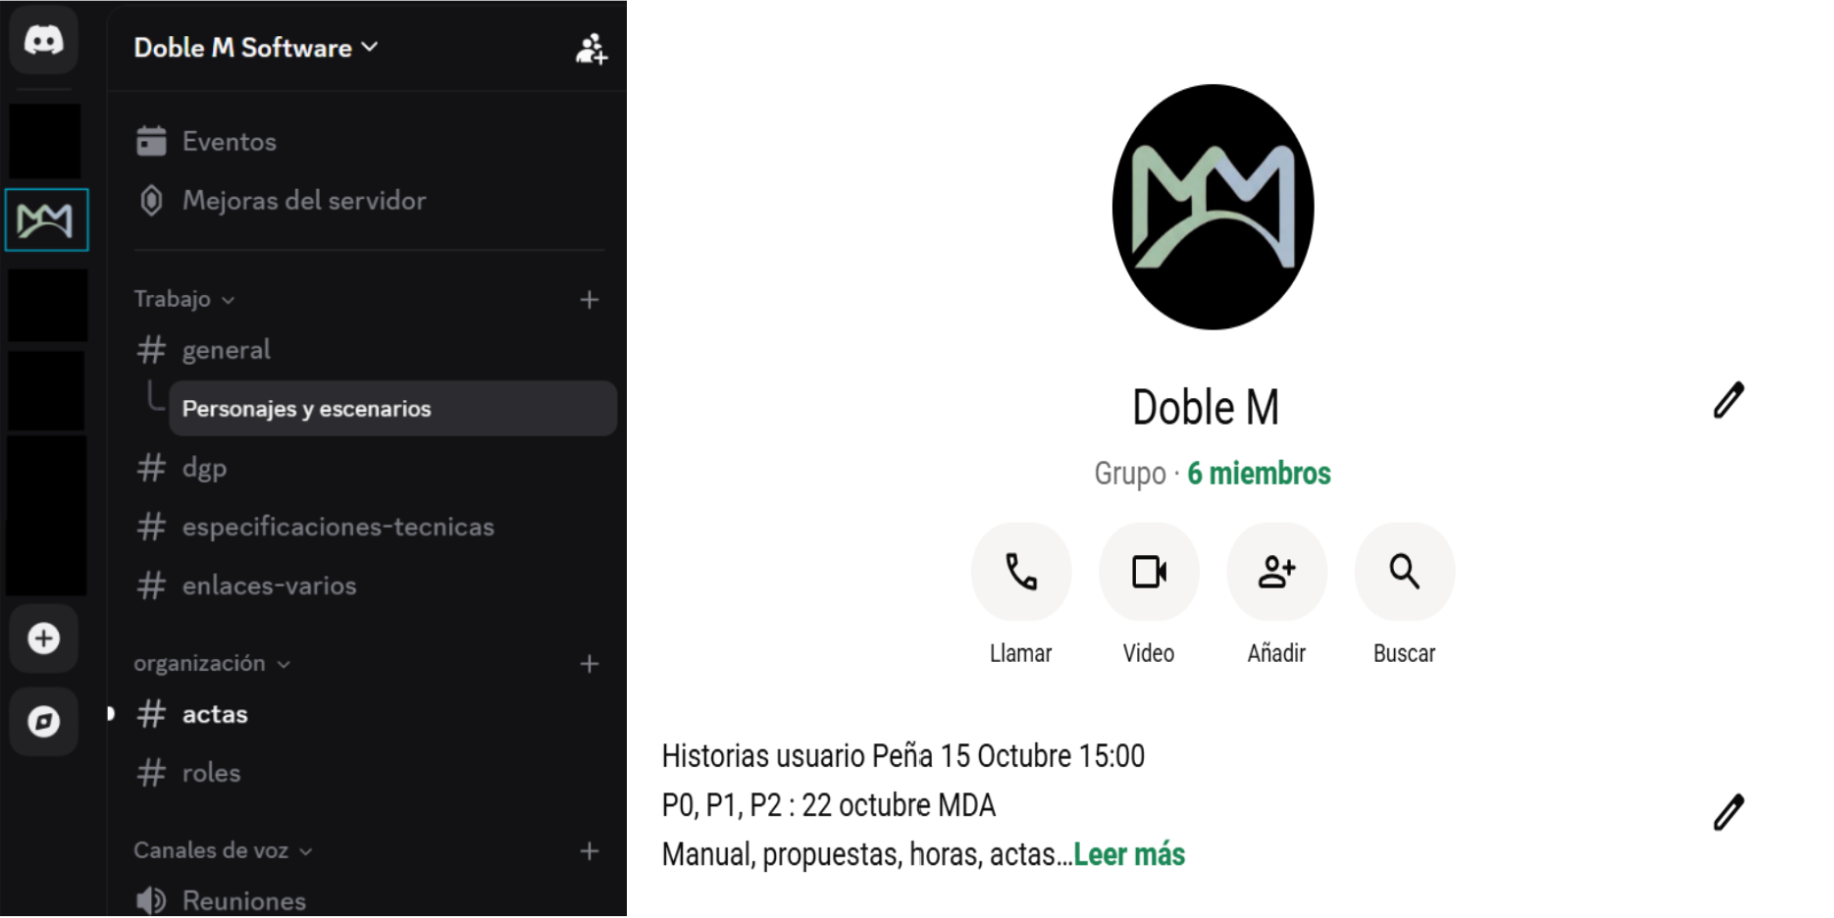
\includegraphics[width=0.8\textwidth]{img/grupo_comunicacion.png}
    \caption{Foto del grupo de WhatsApp y Discord del equipo de trabajo.}
    \label{fig:grupo_comunicacion}
\end{figure}

Estas herramientas se emplearán para resolver dudas rápidas, comunicar incidencias, coordinar reuniones y avisar de cambios que puedan afectar al trabajo de los demás integrantes.

Las reuniones de coordinación servirán para revisar el estado de las tareas, identificar bloqueos, acordar prioridades y organizar el trabajo pendiente.

Además, para tener un seguimiento de los documentos y los elementos básicos para la coordinación y estandarización de los documentos, empleamos GitHub.
\begin{figure}[htbp]
    \centering
    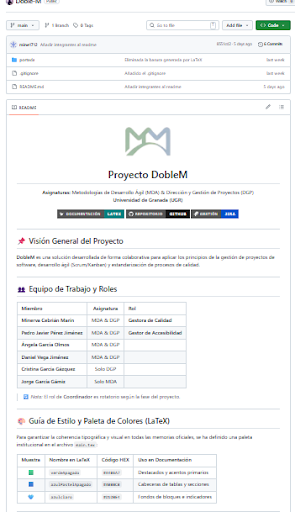
\includegraphics[width=0.8\textwidth]{img/github.png}
    \caption{Foto del repositorio de Github.}
    \label{fig:repo_github}
\end{figure}


\subsection{Relaciones con el Cliente (Entrevistas, Reuniones, Revisiones, \dots)}

La relación con el cliente y con el profesorado se establecerá mediante entrevistas, reuniones de seguimiento y comunicaciones por correo electrónico, para formular consultas concretas o enviar alguna información.

Después de cada reunión o entrevista, se recogerán los aspectos tratados, los acuerdos alcanzados, y las dudas pendientes y cuando sea necesario, se actualizarán los requisitos y las tareas a realizar.

Los cambios solicitados por el cliente se evaluarán teniendo en cuenta su prioridad, su impacto sobre las funcionalidades existentes, el esfuerzo necesario y los plazos de entrega.

% -----------------------------------------------------------------
% ESTÁNDARES
% -----------------------------------------------------------------
\subsection{Estándares de Documentación}

La documentación del proyecto se elaborará utilizando \LaTeX, con el objetivo de mantener un formato uniforme y facilitar su revisión y mantenimiento, siguiendo las siguientes normas:

\begin{itemize}
    \item Los documentos tendrán una portada común con el nombre del equipo y logo, las asignaturas, los integrantes del equipo y la fecha.
    \item Se utilizarán los colores corporativos establecidos.
    \item Se empleará una estructura común de títulos, apartados, tablas, figuras y referencias.
    \item Los archivos fuente se conservarán en formato .tex y las versiones finales se generarán en PDF.
    \item Las figuras y capturas tendrán un título o pie explicativo y se numerarán cuando corresponda.
    \item Se utilizará un lenguaje claro, preciso y coherente en todos los documentos.
    \item Los documentos se guardarán en las carpetas acordadas y se mantendrá un control de sus versiones.
\end{itemize}

\subsection{Estándares de Código}

El código del proyecto seguirá unos estándares comunes para facilitar su lectura, mantenimiento y revisión por parte de todos los integrantes, donde se aplicarán las siguientes normas:

\begin{itemize}
    \item Los comentarios explicativos del código se escribirán en español, mientras que los nombres de variables, funciones, clases y otros identificadores se escribirán en inglés.
    \item Las variables y funciones utilizarán el formato \texttt{camelCase}.
    \item Las clases utilizarán el formato \texttt{PascalCase}.
    \item Las constantes utilizarán el formato \texttt{UPPER\_SNAKE\_CASE}.
    \item Cada función tendrá una responsabilidad concreta y se evitarán funciones excesivamente largas o con demasiadas responsabilidades.
    \item Se evitará duplicar código mediante la reutilización de funciones, siempre que sea posible.
    \item Se utilizarán nombres descriptivos que permitan comprender la finalidad de las variables y funciones.
    \item Se evitará introducir cambios que no estén relacionados con la tarea asignada, salvo que sean necesarios y se comuniquen al equipo.
\end{itemize}

Cuando se incorporen nuevas funcionalidades o se modifique código existente, se realizarán las pruebas que correspondan. Los errores detectados deberán corregirse o registrarse como tareas pendientes en Jira.

% -----------------------------------------------------------------
% GESTIÓN DE CAMBIOS Y CONTROL DE VERSIONES
% -----------------------------------------------------------------
\subsection{Plan de Gestión de Cambios}

Cualquier cambio que afecte a los requisitos, las funcionalidades, el diseño, la planificación o la tecnología deberá comunicarse a todo el equipo y el procedimiento a seguir será el siguiente:

\begin{enumerate}
    \item Se describirá el cambio solicitado o la necesidad detectada.
    \item Se analizará su prioridad y el esfuerzo necesario que requerirá sobre el trabajo ya realizado.
    \item El equipo determinará si el cambio se incorpora a la iteración actual, se planifica para una iteración posterior o se descarta justificadamente.
    \item Si se acepta, se modificarán los requisitos, las tareas, la planificación y la documentación afectada.
    \item Se comprobará que la modificación funciona correctamente y que no ha perjudicado a otras funcionalidades.
\end{enumerate}

Si un integrante no puede completar una tarea asignada, deberá comunicarlo lo antes posible. El equipo valorará la posibilidad de prestar apoyo, reasignar la tarea o dividirla en partes más pequeñas, procurando mantener una distribución equilibrada del trabajo.

\subsection{Control de Versiones (Método y Herramientas)}

El control de versiones se realizará mediante Git y GitHub. El repositorio contendrá el código fuente y los archivos de configuración y documentación.

% -----------------------------------------------------------------
% CALIDAD, DESEMPEÑO Y RECOMPENSAS
% -----------------------------------------------------------------
\subsection{Gestión de Calidad (Durante el Desarrollo y al Final, Incluir Herramientas)}

La gestión de la calidad se realizará durante todo el desarrollo y no únicamente al finalizar el proyecto. Su objetivo será comprobar que el producto cumple los requisitos acordados, que funciona correctamente y que la documentación es coherente con la implementación.

Se llevarán a cabo las siguientes actividades:

\begin{itemize}
    \item Comprobar que las funcionalidades implementadas corresponden con los requisitos e historias de usuario acordados.
    \item Utilizar Jira para comprobar el estado de las tareas, detectar retrasos e identificar trabajo pendiente.
    \item Comprobar la legibilidad, la coherencia con los estándares establecidos y la ausencia de errores.
    \item Verificar que las funcionalidades principales se comportan como se espera.
    \item Verificar que los documentos estén actualizados y tengan un formato común.
    \item Registrar los errores detectados, asignarles prioridad y comprobar su resolución.
\end{itemize}

El Gestor de Calidad coordinará estas actividades y registrará las incidencias relevantes. No obstante, todos los integrantes serán responsables de revisar la calidad de su propio trabajo y de colaborar en las comprobaciones comunes.

\subsection{Plan de Medición del Desempeño, Recompensas}

El seguimiento del desempeño se basará en criterios objetivos relacionados con el trabajo realizado, el cumplimiento de los compromisos y la colaboración con el equipo.

Si un integrante tiene dificultades para completar su trabajo, el equipo analizará las causas y acordará medidas de apoyo o una redistribución de tareas. Si se detecta un incumplimiento reiterado sin comunicación ni justificación, se hablará con la persona implicada y se documentarán los acuerdos de mejora. Si el problema persiste, se informará al profesorado.

Cuando un integrante asuma una carga de trabajo superior a la prevista, se tendrá en cuenta en la planificación posterior para procurar un reparto equilibrado y evitar la sobrecarga.

Como incentivo colectivo, el equipo propone celebrar el logro de una calificación de sobresaliente mediante una actividad de ocio acordada por todos los miembros, como una visita a un parque de atracciones o a un centro recreativo.
% \newpage
% \section{Propuesta Técnica}

\subsection{Título y Resumen}
El proyecto consiste en el análisis, diseño y desarrollo de una aplicación digital que facilite la organización del tiempo y la realización autónoma de actividades cotidianas principalmente a estudiantes con discapacidad intelectual, especialmente a aquellos que participan en el Programa de Transición a la Vida Adulta (PTVAL) del Colegio de Educación Especial Fundación Purísima Concepción de Granada. La aplicación permitirá consultar una agenda personalizada, visualizar las actividades programadas y acceder a instrucciones adaptadas a las necesidades de cada estudiante.

La solución incorporará distintos perfiles de usuario y opciones de personalización de la interfaz, como el tamaño y tipo de letra, los colores y los elementos visuales empleados. También permitirá gestionar actividades, consultar sus detalles y registrar su inicio, progreso y finalización. De esta forma, se pretende facilitar la comprensión de las tareas, favorecer la autonomía del alumnado y mejorar la coordinación entre estudiantes, tutores y profesores. El desarrollo se realizará siguiendo la metodología Scrum, mediante tres iteraciones, y prestando especial atención a la accesibilidad, la usabilidad y la protección de los datos personales.

\subsection{Duración en Meses}
El proyecto se desarrollará desde el 25 de septiembre de 2026 hasta el 21 de diciembre de 2026. Su duración total será de aproximadamente tres meses, incluyendo la preparación inicial, las tres iteraciones de desarrollo y las actividades de cierre y documentación final.

\subsection{Tipo de Caso de Negocio}
El proyecto responde principalmente a una demanda de un cliente, el Colegio de Educación Especial Fundación Purísima Concepción de Granada, que necesita una herramienta digital para facilitar la organización del tiempo y promover la autonomía de estudiantes con discapacidad intelectual.

La iniciativa también responde a una necesidad de mejora de accesibilidad, ya que las soluciones existentes no siempre se adaptan suficientemente a las capacidades cognitivas, preferencias y necesidades de cada estudiante. Por tanto, se propone desarrollar una aplicación que facilite la personalización de las agendas y simplifique la gestión de actividades por parte de los tutores y profesores.

\subsection{Objetivos}

\subsubsection{Objetivo General}
Diseñar, desarrollar y verificar una aplicación web accesible y personalizable que facilite la planificación y realización de actividades escolares y personales de estudiantes con discapacidad intelectual, permitiendo su gestión y seguimiento por parte de los propios estudiantes, sus tutores y los profesores autorizados.

\subsubsection{Objetivos Específicos}
\definecolor{verdeTag}{HTML}{2E7D32}
\definecolor{amarilloTag}{HTML}{E65100}
\definecolor{grisTag}{HTML}{616161}

\paragraph{Requisitos Funcionales (RF)}
Definen las funcionalidades que deberá proporcionar la aplicación. A continuación se detalla su alcance y nivel de cobertura en el proyecto:

\begin{xltabular}{\textwidth}{|p{2.2cm}|X|p{2.8cm}|}
\hline
\rowcolor{azulPastelApagado}
\textbf{Código} & \textbf{Descripción del Requisito Funcional} & \textbf{Estado / Alcance} \\ \hline
\endhead

\hline
\endfoot

\rowcolors{2}{azulclaro}{white}
\textbf{RF1} & Implementar un sistema de inicio de sesión que permita a cada usuario acceder a las funcionalidades correspondientes a su perfil. & \cellcolor{verdeApagado}\textbf{Incluido} \\ \hline
\textbf{RF2} & Permitir al profesor consultar los estudiantes que tiene asignados y seleccionar uno para acceder a su información. & \cellcolor{verdeApagado}\textbf{Incluido} \\ \hline
\textbf{RF3} & Permitir al administrador gestionar cuentas de estudiantes, profesores y tutores. & \cellcolor{verdeApagado}\textbf{Incluido} \\ \hline
\textbf{RF3.1} & --- Crear cuentas de estudiantes, profesores y tutores. & \cellcolor{verdeApagado}\textbf{Incluido} \\ \hline
\textbf{RF3.2} & --- Eliminar cuentas de estudiantes, profesores y tutores. & \cellcolor{verdeApagado}\textbf{Incluido} \\ \hline
\textbf{RF3.3} & --- Establecer relaciones entre estudiantes, profesores y tutores legales. & \cellcolor{verdeApagado}\textbf{Incluido} \\ \hline
\textbf{RF3.4} & --- Editar cuentas de estudiantes, profesores y tutores. & \cellcolor{verdeApagado}\textbf{Incluido} \\ \hline
\textbf{RF5} & Permitir a la familia consultar el perfil de un estudiante. & \cellcolor{verdeApagado}\textbf{Incluido} \\ \hline
\textbf{RF6} & Permitir a la Familia consultar y editar sus preferencias de configuración. & \cellcolor{verdeApagado}\textbf{Incluido} \\ \hline
\textbf{RF7} & Permitir al estudiante sus preferencias de configuración. & \cellcolor{verdeApagado}\textbf{Incluido} \\ \hline
\textbf{RF7.1} & --- Preferencias de texto (Tamaño, pictogramas, contraste). & \cellcolor{verdeApagado}\textbf{Incluido} \\ \hline
\textbf{RF7.1.1} & ------ Mostrar pictogramas en lugar de texto plano. & \cellcolor{verdeApagado}\textbf{Incluido} \\ \hline
\textbf{RF7.1.2} & ------ Permitir inputs de texto mediante voz. & \textit{Opcional} \\ \hline
\textbf{RF7.1.3} & ------ Preferencias de contraste. & \cellcolor{verdeApagado}\textbf{Incluido} \\ \hline
\textbf{RF7.1.4} & ------ Preferencias de tamaño de texto. & \cellcolor{verdeApagado}\textbf{Incluido} \\ \hline
\textbf{RF7.1.5} & ------ Preferencias respecto al tiempo. & \cellcolor{verdeApagado}\textbf{Incluido} \\ \hline
\textbf{RF7.2} & --- Preferencias de colores de la aplicación. & \cellcolor{verdeApagado}\textbf{Incluido} \\ \hline
\textbf{RF8} & Permitir al estudiante cambiar su imagen de perfil de usuario. & \cellcolor{verdeApagado}\textbf{Incluido} \\ \hline
\textbf{RF9} & Mostrar al estudiante las actividades programadas para un día seleccionado. & \cellcolor{verdeApagado}\textbf{Incluido} \\ \hline
\textbf{RF10} & Mostrar al estudiante consultar las actividades de la semana. & \cellcolor{verdeApagado}\textbf{Incluido} \\ \hline
\textbf{RF11} & Consultar detalles de una actividad (imagen, descripción, horario, instrucciones). & \cellcolor{verdeApagado}\textbf{Incluido} \\ \hline
\textbf{RF11.1} & --- Permitir al profesor acceder a la lista de estudiantes participantes. & \cellcolor{verdeApagado}\textbf{Incluido} \\ \hline
\textbf{RF12} & Crear actividades personales y escolares indicando detalles completos. & \cellcolor{verdeApagado}\textbf{Incluido} \\ \hline
\textbf{RF13} & Editar y cancelar actividades propias actualizando las agendas afectadas. & \cellcolor{verdeApagado}\textbf{Incluido} \\ \hline
\textbf{RF14} & Permitir a la familia editar/cancelar actividades creadas por el estudiante. & \cellcolor{verdeApagado}\textbf{Incluido} \\ \hline
\textbf{RF15} & Permitir al profesor asignar actividades a grupos o estudiantes concretos. & \cellcolor{verdeApagado}\textbf{Incluido} \\ \hline
\textbf{RF16} & Permitir al estudiante confirmar el inicio y la finalización de una actividad. & \cellcolor{verdeApagado}\textbf{Incluido} \\ \hline
\textbf{RF17} & Marcar individualmente los pasos de una actividad completada en secuencia. & \cellcolor{verdeApagado}\textbf{Incluido} \\ \hline
\textbf{RF18} & Configurar la visualización de un reloj/indicador de tiempo en actividades. & \cellcolor{verdeApagado}\textbf{Incluido} \\ \hline
\textbf{RF19} & Permitir al estudiante recibir avisos del comienzo de actividades. & \cellcolor{verdeApagado}\textbf{Incluido} \\ \hline
\textbf{RF20} & Incorporar un canal de comunicación accesible entre estudiante y tutores. & No incluido \\ \hline
\textbf{RF21} & Proponer actividades optativas automáticas si una tarea se cancela. & No incluido \\ \hline
\textbf{RF22} & Valorar actividades realizadas para personalizar futuras sugerencias. & No incluido \\ \hline
\textbf{RF23} & Avisar al estudiante cuando una actividad asignada sea cancelada. & \textit{Opcional} \\ \hline
\textbf{RF24} & Bloqueo de inicio de sesión tras 5 intentos fallidos en 2 minutos. & \cellcolor{verdeApagado}\textbf{Incluido} \\ \hline
\end{xltabular}

\vspace{0.6cm}

\paragraph{Requisitos No Funcionales (RNF)}
Definen las condiciones de calidad, accesibilidad, seguridad y funcionamiento que deberá cumplir la aplicación.

\begin{table}[H]
\centering
\rowcolors{1}{white}{white}
\begin{tabularx}{\textwidth}{|p{2.2cm}|X|}
\hline
\rowcolor{azulPastelApagado}
\textbf{Código} & \textbf{Criterios de Calidad y Usabilidad} \\ \hline
\rowcolor{azulclaro}
\textbf{RNF1} & Diseñar una interfaz sencilla, consistente y comprensible, reduciendo la cantidad de información y opciones mostradas simultáneamente al estudiante. \\ \hline
\textbf{RNF2} & Permitir adaptar la presentación de la aplicación a las necesidades individuales mediante las opciones de personalización disponibles. \\ \hline
\rowcolor{azulclaro}
\textbf{RNF3} & Utilizar textos claros y concisos, instrucciones breves, iconos comprensibles y apoyos visuales adecuados para facilitar la comprensión de las actividades. \\ \hline
\textbf{RNF4} & Facilitar la interacción mediante controles suficientemente grandes, una disposición clara de los elementos y una navegación sencilla, teniendo en cuenta las necesidades de movilidad de los usuarios. \\ \hline
\rowcolor{azulclaro}
\textbf{RNF5} & Garantizar que las funcionalidades principales puedan utilizarse desde los navegadores y dispositivos compatibles definidos para el proyecto. \\ \hline
\textbf{RNF6} & Proteger el acceso a la información mediante autenticación y comprobación de permisos según el perfil del usuario. \\ \hline
\rowcolor{azulclaro}
\textbf{RNF7} & Garantizar que los usuarios solo puedan consultar o modificar la información para la que tengan autorización. \\ \hline
\textbf{RNF8} & Aplicar medidas de protección de datos personales, limitando la información recogida a la necesaria y cumpliendo la normativa aplicable. \\ \hline
\rowcolor{azulclaro}
\textbf{RNF9} & Diseñar e implementar paletas de colores coherentes para mostrar en la aplicación. \\ \hline
\textbf{RNF10} & Diseñar una página de login accesible. \\ \hline
\end{tabularx}
\end{table}

\vspace{0.6cm}

\paragraph{Requisitos de Implementación (RI)}
Definen las tecnologías, herramientas y condiciones técnicas previstas para desarrollar y ejecutar la solución.

\begin{table}[H]
\centering
\rowcolors{1}{white}{white}
\begin{tabularx}{\textwidth}{|p{2.2cm}|X|}
\hline
\rowcolor{azulPastelApagado}
\textbf{Código} & \textbf{Especificación Técnica / Restricción de Dominio} \\ \hline
\rowcolor{azulclaro}
\textbf{RI1} & Respecto de los usuarios se debe almacenar: correo, nombre de usuario, nombre real, fecha de nacimiento. \\ \hline
\textbf{RI2} & Cuando una cuenta es dada de baja, sus datos permanecen almacenados al menos 4 años. \\ \hline
\rowcolor{azulclaro}
\textbf{RI3} & Los usuarios pertenecen a una de las siguientes categorías: Estudiante, Profesor, Familia o Administrador. \\ \hline
\textbf{RI4} & Los usuarios deben poder seleccionar sus preferencias de personalización y estas deben permanecer entre sesión y sesión. \\ \hline
\rowcolor{azulclaro}
\textbf{RI5} & Las actividades deben tener una descripción que puede componerse de texto, imágenes o videos. \\ \hline
\textbf{RI6} & Las actividades pueden contener varios pasos personalizables y verificables individualmente. \\ \hline
\rowcolor{azulclaro}
\textbf{RI7} & Las actividades deben almacenar su estado de “sin empezar/comenzada/terminada”. \\ \hline
\textbf{RI8} & Los estudiantes pueden tener actividades asignadas en una fecha concreta con una hora de inicio y fin dadas. \\ \hline
\rowcolor{azulclaro}
\textbf{RI9} & Los profesores y la familia pueden crear actividades para asignarlas a los estudiantes. \\ \hline
\textbf{RI10} & Los estudiantes podrán estar relacionados con profesores y familia de forma específica. \\ \hline
\rowcolor{azulclaro}
\textbf{RI11} & Los estudiantes pueden pertenecer a grupos de clase. \\ \hline
\textbf{RI12} & Uno o varios profesores pueden enviar tareas a un grupo de estudiantes. \\ \hline
\rowcolor{azulclaro}
\textbf{RI13} & Las contraseñas deben ser cifradas a la hora de almacenarlas. \\ \hline
\end{tabularx}
\end{table}

\subsection{Antecedentes del Equipo de Trabajo}
El equipo está formado por seis estudiantes de último año con formación en Ingeniería Informática, los cuales contamos con conocimientos en distintas áreas, lenguajes de programación y herramientas de desarrollo que nos permiten afrontar el análisis, diseño, programación y pruebas del sistema exigidas.

Dado que no todos tenemos la misma experiencia previa en desarrollo web, reservaremos un tiempo inicial para formarnos e igualar el nivel técnico del grupo. Además, aunque tenemos una base sólida en distintas áreas de trabajo, esta es nuestra primera experiencia trabajando en un equipo de desarrollo con un enfoque similar al profesional. Por ello, nos organizaremos bien a la hora de coordinarnos, repartirnos las tareas, gestionar el control de versiones y revisar el trabajo, asegurando así una buena colaboración y un resultado de calidad.

\subsection{Justificación: Revisión de Soluciones Relacionadas con la Temática Comparativa}
Existen aplicaciones y recursos que permiten organizar actividades mediante agendas visuales, imágenes y pictogramas. Algunas de ellas son las siguientes:

\begin{itemize}
    \item \textbf{PictogramAgenda:} Permite crear secuencias ordenadas de pictogramas, destacar la actividad actual, marcar tareas realizadas y utilizar sonido y temporizadores.
    \item \textbf{Día a Día:} Ofrece un diario visual para registrar y anticipar actividades mediante imágenes, fotografías, vídeos, sonidos y textos, con opciones de personalización.
\end{itemize}
\begin{figure}[htbp]
    \centering
    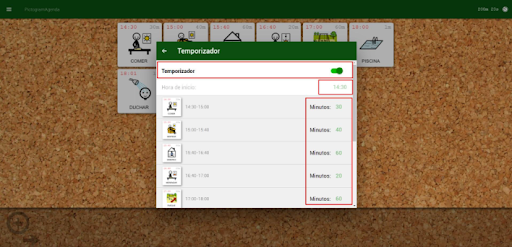
\includegraphics[width=0.8\textwidth]{img/pictograma_agenda.png}
    \caption{Foto de PictogramAgenda}
    \label{fig:pictogram_agenda}
\end{figure}
\begin{figure}[htbp]
    \centering
    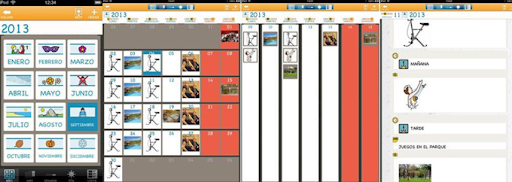
\includegraphics[width=0.8\textwidth]{img/dia_a_dia.png}
    \caption{Foto de Dia a Dia Agenda.}
    \label{fig:dia_a_dia_agenda}
\end{figure}

A continuación, vamos a realizar una comparativa de las agendas que hay en el mercado con la propuesta que se nos ofrece, para ver en qué se diferencia y qué aspectos añaden valor a nuestra agenda con respecto a otras opciones propuestas en el mercado.

\begin{table}[H]
\centering
\rowcolors{2}{azulclaro}{white}
\begin{tabularx}{\textwidth}{X p{2.8cm} p{2.8cm} p{3.2cm}}
\toprule
\rowcolor{azulPastelApagado}
\textbf{Característica} & \textbf{PictogramAgenda} & \textbf{Día a Día} & \textbf{Agenda Doble} \\
\midrule
Organización visual de actividades & Sí & Sí & Sí \\
Imágenes y pictogramas & Sí & Sí & Sí \\
Personalización visual & Algunas opciones & Sí & Orientada a cada perfil \\
Gestión de perfiles de estudiante y tutor & No es su función principal & No es su función principal & Sí \\
Asignación y seguimiento de actividades escolares & Limitado al uso de la agenda visual & No es su función principal & Sí \\
Gestión de actividades personales & Sí, mediante secuencias & Sí, mediante diario visual & Sí \\
\bottomrule
\end{tabularx}
\caption{Comparativa de soluciones existentes frente a Agenda Doble.}
\end{table}

En definitiva, aunque ya existen herramientas que ofrecen buenas funciones para organizar actividades visualmente, nuestro objetivo es unificar la gestión de usuarios, perfiles personalizados y un control completo de las tareas escolares y personales en nuestra aplicación, siendo lo más personalizable posible y adaptado al día a día del estudiante.

\subsection{Descripción y Esquema de Solución}
\textit{(CREO QUE ESTA ES LA PROPUESTA DE SOLUCIÓN)}

La solución consistirá en una aplicación web accesible y adaptable a distintos dispositivos, destinada principalmente a estudiantes del PTVAL y a las personas autorizadas que les acompañan. La aplicación organizará sus funcionalidades según el perfil del usuario, evitando mostrar opciones innecesarias y facilitando una interacción sencilla.

El estudiante podrá consultar su agenda, visualizar la información de las actividades, acceder a instrucciones adaptadas, marcar los pasos realizados y confirmar el inicio y la finalización de las tareas. Según la configuración disponible, podrá consultar actividades de los próximos días, personalizar sus preferencias y crear actividades personales.

Los tutores y profesores podrán gestionar las actividades de los estudiantes que tengan asignados, consultar sus perfiles y realizar un seguimiento de su progreso. El administrador se encargará de gestionar las cuentas y las relaciones entre usuarios. Las funcionalidades se implementarán de forma progresiva, atendiendo a la prioridad de las historias de usuario y al tiempo disponible.

\subsubsection{Tecnologías Previstas}
\begin{itemize}
    \item \textbf{HTML:} estructura de las páginas.
    \item \textbf{CSS:} presentación visual y adaptación de la interfaz a diferentes necesidades.
    \item \textbf{JavaScript:} interacciones y funcionalidades del lado del cliente.
    \item \textbf{PHP:} lógica del servidor, validación de peticiones y comunicación con la base de datos.
    \item \textbf{MySQL:} almacenamiento de usuarios, perfiles, actividades y registros de seguimiento.
    \item \textbf{Docker:} ejecución de los servicios en contenedores.
    \item \textbf{Git y GitHub:} control de versiones y trabajo compartido.
\end{itemize}

\subsubsection{Arquitectura Propuesta}
La aplicación seguirá una arquitectura web cliente-servidor organizada en tres niveles: interfaz de usuario, lógica de aplicación y almacenamiento de datos.

\begin{enumerate}
    \item \textbf{Presentación:} el navegador mostrará la interfaz desarrollada con HTML, CSS y JavaScript.
    \item \textbf{Lógica de aplicación:} el servidor PHP gestionará la autenticación, los permisos, las operaciones sobre las actividades y las solicitudes de los usuarios.
    \item \textbf{Persistencia:} MySQL almacenará la información necesaria para el funcionamiento del sistema.
    \item \textbf{Despliegue:} Docker permitirá configurar y ejecutar los servicios necesarios de forma organizada.
\end{enumerate}

\paragraph{Esquema general:}
Usuario $\rightarrow$ Interfaz web (HTML, CSS y JavaScript) $\rightarrow$ Servidor PHP $\rightarrow$ Base de datos MySQL

\vspace{0.3cm}
Docker facilitará la ejecución de los componentes y GitHub permitirá mantener el código y su historial de cambios.

La aplicación deberá diseñarse teniendo en cuenta la accesibilidad cognitiva, visual y motora, así como la protección de los datos personales. Se priorizarán las instrucciones claras, los elementos visuales comprensibles, los controles fáciles de utilizar y la adaptación de la interfaz a cada perfil. La solución definitiva se concretará a partir de los requisitos acordados con el cliente y de las pruebas realizadas durante el desarrollo.

\subsection{Actividades a Realizar}
Las actividades se organizan provisionalmente en función de los objetivos específicos del proyecto. Su distribución definitiva se ajustará a la planificación acordada por el equipo.

\begin{table}[H]
\centering
\rowcolors{2}{azulclaro}{white}
\begin{tabularx}{\textwidth}{p{4.5cm} p{3.2cm} X}
\toprule
\rowcolor{azulPastelApagado}
\textbf{Actividad} & \textbf{Objetivos} & \textbf{Resultado esperado} \\
\midrule
A1. Análisis de requisitos y necesidades del cliente & 1, 2 & Especificación de requisitos e historias de usuario. \\
A2. Diseño de la interfaz y de la arquitectura & 2, 8 & Prototipos, diseño de la base de datos y arquitectura del sistema. \\
A3. Implementación de usuarios y perfiles & 4, 7 & Gestión de cuentas, permisos y preferencias. \\
A4. Desarrollo de la agenda y las actividades & 3, 4, 5, 6 & Consulta y gestión de actividades personales y escolares. \\
A5. Implementación de la personalización y accesibilidad & 2, 5, 8 & Interfaz adaptada a las necesidades de los usuarios. \\
A6. Pruebas y evaluación de calidad & 8, 9 & Registro de pruebas, incidencias y correcciones. \\
A7. Gestión y documentación del proyecto & 10 & Documentación actualizada, seguimiento y entregas. \\
\bottomrule
\end{tabularx}
\caption{Matriz de actividades, objetivos y resultados esperados.}
\end{table}

\subsection{Cronograma}

El proyecto seguirá una planificación basada en una fase inicial y tres iteraciones de desarrollo. Las fechas siguientes corresponden a la planificación proporcionada por el equipo.

\begin{table}[H]
\centering
\rowcolors{2}{azulclaro}{white}
\begin{tabularx}{\textwidth}{p{3cm} p{3cm} p{3cm} X}
\toprule
\rowcolor{azulPastelApagado}
\textbf{Fase} & \textbf{Inicio} & \textbf{Entrega prevista} & \textbf{Principales resultados} \\
\midrule
Iteración 0 & Fase inicial & 21-22 oct 2026 & Manual de coordinación, propuesta técnica y documentación inicial. \\
Iteración 1 & 22-23 oct 2026 & 11-12 nov 2026 & Primer incremento funcional y presentación de la iteración. \\
Iteración 2 & 12-13 nov 2026 & 2-3 dic 2026 & Segundo incremento, pruebas y presentación de resultados. \\
Iteración 3 & 3-4 dic 2026 & 21 dic 2026 & Incremento final previsto, pruebas y documentación asociada. \\
Cierre del proyecto & Tras iteración 3 & 6 feb 2027 & Revisión final, documentación pendiente y entrega definitiva. \\
\bottomrule
\end{tabularx}
\caption{Planificación y cronograma por fases e iteraciones.}
\end{table}

\subsection{Implicación de los Participantes}
\begin{itemize}
    \item \textbf{Equipo de desarrollo:} todos los integrantes participarán en el análisis, diseño, implementación, pruebas y documentación, según el reparto de tareas.
    \item \textbf{Coordinadores de cada iteración:} organizarán el trabajo, revisarán el avance y facilitarán la resolución de bloqueos.
    \item \textbf{Gestor de calidad:} supervisará las comprobaciones y el registro de incidencias.
    \item \textbf{Gestor de usabilidad y accesibilidad:} revisará la adecuación de la interfaz y las funcionalidades a las necesidades del alumnado.
    \item \textbf{Cliente y profesorado:} aportarán información sobre las necesidades, revisarán los avances y ayudarán a validar los requisitos.
\end{itemize}

La distribución concreta de funcionalidades y entregables por iteración se establecerá en el Product Backlog y en la planificación de cada iteración. Las fechas y los hitos intermedios deberán actualizarse si el profesorado establece otras condiciones.

\subsection{Cauces de Seguimiento}
El seguimiento del proyecto se realizará mediante reuniones periódicas con el profesorado o con el cliente. La comunicación formal con el mismo se realizará principalmente mediante correo electrónico para concertar reuniones mínimo una vez por iteración, donde se revisarán los avances, resolveremos dudas y validaremos las decisiones relacionadas con los requisitos.

Después de cada reunión se elaborarán actas en las que se recogerán los temas tratados, los acuerdos alcanzados y las cuestiones pendientes. Si el cliente solicita cambios, se analizará su prioridad, el esfuerzo necesario y su impacto sobre la planificación antes de incorporarlos al proyecto.

Para el seguimiento interno, se utilizará Jira, donde se registrarán las tareas, sus responsables y su estado. GitHub permitirá consultar la evolución del código y la documentación compartida. Además, el equipo mantendrá una comunicación continua mediante Discord y/o WhatsApp para resolver dudas y comunicar incidencias.

Al finalizar cada iteración se revisará el incremento desarrollado, se comprobará el cumplimiento de los objetivos previstos y se identificarán las mejoras necesarias para la siguiente fase.

\subsection{Valor Añadido}


Además de las funcionalidades básicas descritas en el pliego, la aplicación pretende aportar los siguientes elementos de valor añadido:

\begin{itemize}
    \item \textbf{Personalización centrada en el usuario:} adaptación de los elementos visuales y de la presentación de la agenda según las necesidades de cada estudiante.
    \item \textbf{Integración de actividades escolares y personales:} posibilidad de reunir en una misma herramienta las tareas asignadas en el centro y las actividades cotidianas.
    \item \textbf{Seguimiento del progreso:} consulta del estado de las actividades para facilitar el acompañamiento educativo.
    \item \textbf{Diseño modular:} organización de las funcionalidades por perfiles para facilitar su adaptación a las necesidades del centro.
    \item \textbf{Accesibilidad como criterio transversal:} consideración de las necesidades cognitivas, visuales y motoras desde el análisis hasta las pruebas finales.
    \item \textbf{Posible reutilización fuera del centro:} diseño de una herramienta que también pueda utilizarse como agenda personal por otros usuarios.
\end{itemize}

Las funcionalidades adicionales, como el chat accesible, las sugerencias de actividades alternativas o la valoración de tareas, se considerarán mejoras potenciales sujetas a la prioridad acordada y a la capacidad de desarrollo del equipo.

\subsection{Beneficios y Beneficiarios}

\subsubsection{Beneficiarios Directos}
\begin{itemize}
    \item \textbf{Estudiantes del PTVAL con discapacidad intelectual:} podrán consultar sus actividades de forma estructurada y adaptada a sus necesidades, favoreciendo su autonomía y participación en las tareas cotidianas.
    \item \textbf{Profesores y tutores del centro:} dispondrán de una herramienta para organizar actividades, asignarlas y consultar su estado.
    \item \textbf{Tutores legales y familiares:} podrán colaborar en la planificación de las actividades personales de los estudiantes que tengan asignados, dentro de los permisos establecidos.
\end{itemize}

\subsubsection{Beneficiarios Indirectos}
\begin{itemize}
    \item \textbf{Colegio de Educación Especial Fundación Purísima Concepción de Granada:} podrá disponer de una herramienta adaptada a sus necesidades educativas y organizativas.
    \item \textbf{Otros usuarios con necesidades de organización o accesibilidad:} podrán beneficiarse de las funciones de agenda y personalización, siempre que la solución final se adapte a sus necesidades.
\end{itemize}

\subsubsection{Beneficios Esperados}
El proyecto pretende favorecer la autonomía de los estudiantes, facilitar la comprensión de las actividades, reducir la complejidad de la planificación para los tutores y mejorar la coordinación entre el entorno educativo y familiar. Asimismo, permitirá al equipo aplicar conocimientos de ingeniería informática y gestión de proyectos en un contexto real de aprendizaje-servicio.

En cuanto a la propiedad intelectual, los productos y documentos resultantes serán de autoría compartida entre el equipo de trabajo y los peticionarios, de acuerdo con lo establecido en el pliego técnico.
% \newpage
%\include{cap/dgp/cliente/jira}
\newpage
%\section{Propuesta de Solución}

La propuesta consiste en desarrollar una aplicación web llamada Doble Agenda para el alumnado con discapacidad intelectual del centro Fundación Purísima Concepción de Granada. Su objetivo es ayudar a sus alumnos a organizar sus actividades diarias y escolares, consultar qué tareas tienen pendientes y seguir los pasos necesarios para poder completarlas. Además, permitirá que los profesores organicen las actividades y que las familias puedan también consultar la información del alumno.

\subsection{Funcionalidades que sí se van a desarrollar}
En primer lugar, la aplicación contará con diferentes perfiles de usuario: administrador, profesor, familiar y alumno. Cada uno tendrá acceso a las funciones que le correspondan. Se incluirá la gestión de cuentas y permisos, además de la posibilidad de que los profesores puedan consultar a sus alumnos asignados y que las familias puedan acceder a la información de sus propios hijos.

También, se desarrollará una agenda que permita consultar las actividades del día y de la semana, ver sus detalles e instrucciones y crear actividades personales o escolares. Los profesores podrán asignarlas tanto a alumnos individuales como a grupos de clase. Por su parte, los alumnos podrán indicar cuándo empiezan y terminan una actividad y marcar los pasos que hayan completado cuando una tarea esté dividida en varias partes.

Por último, se incluirán opciones de personalización de la interfaz, como la configuración de colores y la posibilidad de cambiar la foto de perfil. Estas funciones buscan que la aplicación resulte más cómoda y fácil de utilizar, adaptándose así en todo lo posible a las preferencias del alumnado.

Se han priorizado este tipo de funcionalidades porque constituyen la base fundamental de la aplicación, además de que permiten facilitar la organización de las actividades y buscan fomentar la autonomía de los alumnos.

\subsection{Funcionalidades opcionales}
Algunas funcionalidades se han considerado opcionales, ya que, aunque pueden llegar a mejorar la experiencia de uso, no son imprescindibles para que la aplicación cumpla con su objetivo principal. Entre ellas se encuentran la edición o cancelación de actividades, los recordatorios y avisos, el indicador de la hora o reloj, las notificaciones de cancelación y algunas opciones adicionales de personalización, como pueden ser modificar el tamaño del texto o introducir texto mediante la voz.

La incorporación de estas funciones dependerá del tiempo disponible y de cómo avance el desarrollo del proyecto. Al tratarse de un trabajo de la universidad, es necesario compaginarlo con otras asignaturas, prácticas y exámenes, por lo que se ha decidido priorizar las funcionalidades esenciales y básicas, y dejar estas mejoras para el caso de que tengamos tiempo suficiente.

\subsection{Funcionalidades que quedan fuera del proyecto}
En principio, se ha decidido no incluir un canal de comunicación entre usuarios, la sugerencia automática de actividades alternativas cuando se cancela una, ni la posibilidad de que los alumnos valoren las actividades generadas por la aplicación.

El motivo principal por el que hemos decidido no añadir estas funcionalidades es porque ampliarían la complejidad del proyecto y no son realmente necesarias para cubrir las necesidades básicas de organización y seguimiento de actividades. Además, requerirían dedicar más tiempo a su diseño e implementación y, teniendo en cuenta el tiempo disponible del grupo y la carga de trabajo de otras asignaturas con prácticas y exámenes, se ha preferido dedicar el tiempo de desarrollo a las funcionalidades que aportan más valor al objetivo principal de la aplicación Doble Agenda. No obstante, en un futuro, podrían estudiarse como posibles mejoras de la aplicación en otras versiones posteriores.

\subsection{Arquitectura de la solución}
Doble Agenda será una aplicación web accesible desde un navegador, sin necesidad de tener que instalar ningún programa. Se utilizará una arquitectura cliente-servidor, en la que el cliente corresponde a la interfaz con la que interactúan los usuarios, mientras que el servidor se encargará de procesar las peticiones y gestionar la información relacionada con los usuarios, las actividades y las agendas.

La aplicación se basará en una interfaz sencilla, intuitiva y adaptada a las necesidades de los distintos perfiles de usuario, facilitando así la navegación y el acceso a las funcionalidades principales.




\end{document}